%%%%%%%%%%%%%%%%%%%%%%%%%%%%%%%%%%%%%%%%% 
% University/School Laboratory Report
% LaTeX Template
% Version 3.1 (25/3/14)
% 
% This template has been downloaded from:
% http://www.LaTeXTemplates.com
% 
% Original author:
% Linux and Unix Users Group at Virginia Tech Wiki 
% (https://vtluug.org/wiki/Example_LaTeX_chem_lab_report)
% 
% License:
% CC BY-NC-SA 3.0 (http://creativecommons.org/licenses/by-nc-sa/3.0/)
% 
%%%%%%%%%%%%%%%%%%%%%%%%%%%%%%%%%%%%%%%%% 

% ----------------------------------------------------------------------------------------
%	PACKAGES AND DOCUMENT CONFIGURATIONS
% ----------------------------------------------------------------------------------------

\documentclass[a4paper, 11pt]{article}

\usepackage{graphicx} % Required for the inclusion of images
\usepackage{epstopdf} % eps to pdf
\usepackage{epsfig}
\usepackage{amsmath} % Required for some math elements 
\usepackage[colorlinks, linkcolor=black, anchorcolor=blue,
citecolor=black]{hyperref}
\usepackage{algorithm}
\usepackage{algpseudocode}
\usepackage{tikz}
\usepackage{pgflibraryarrows}
\usepackage{pgflibrarysnakes}
\usepackage{subfig}
%\usepackage{float}
\usepackage{booktabs} 
\newtheorem{remark}{Remark}[section]
% \setlength\parindent{0pt} % Removes all indentation from paragraphs

% \renewcommand{\labelenumi}{\alph{enumi}.} % Make numbering in the enumerate environment by letter rather than number (e.g. section 6)

% \usepackage{times} % Uncomment to use the Times New Roman font

% ----------------------------------------------------------------------------------------
%	DOCUMENT INFORMATION
% ----------------------------------------------------------------------------------------

\title{Moving mesh finite element method for unsteady Navier-Stokes flow
  } % Title

\author{Yirong Wu and Heyu Wang \\
  \small Department of Mathematics, ZheJiang University, HangZhou,
  310027, China\\
  \small Department of Mathematics, ZheJiang University, HangZhou,
  310027, China }
 % Author name
%\date{\today} % Date for the report

\begin{document}

\maketitle % Insert the title, author and date

% \begin{center}
%   \begin{tabular}{l r}
%     Date Performed: & April 28, 2014 \\ % Date the experiment was performed
%     Partners: & Heyu Wang \\ % Partner names
%     % & Peter Jim \\
%     Instructor: & Professor Heyu Wang \\% Instructor/supervisor
%     Address: & Department of Mathematics, ZheJiang University 
%   \end{tabular}
% \end{center}

% If you wish to include an abstract, uncomment the lines below
% \begin{abstract}
%   Abstract text
% \end{abstract}

% ----------------------------------------------------------------------------------------
%	SECTION 1
% ----------------------------------------------------------------------------------------
\begin{abstract}
    In this paper, we use a $4P1-P1$ finite element pair to solve
    the time-dependent Navier Stokes equations in 2D. This 
    $4P1-P1$ element pair is based on the data structure of hierarchy
    geometry tree. Two-layer nested meshes are used, that velocity
    mesh can be obtained by globally refining pressure mesh. Based on
    this tree structure, we can make the index between elements of
    velocity and pressure. Thus the process to assemble
    divergence matrix is trival with the index. On account of this data
    structure, h-adaptive mesh method can be used. Meanwhile,
    multigrid precondition can be implemented by this data structure. 

    In this work, moving mesh method is applied to solve
    incompressible Navier Stokes equations using $4P1-P1$ finite
    element pair. Seveval numerical problems are used to test the
    moving mesh strategy. \\
    
    Key words: Navier Stokes, $4P1-P1$, multigrid precondition,
    hierarchy geometry tree, moving mesh.

\end{abstract}
% ----------------------------------------------------------------------------------------
%	SECTION 2
% ----------------------------------------------------------------------------------------

\section{Introduction}

    It is important that solving incompressible
    Navier-Stokes equations by mixed finite element method. In order to
    satisfy the LBB condition, one way is to enhance the finite
    element space of velocity relative to pressure, for example 
    Taylor-Hood \cite{taylor1974navier}. The other method is imposing
    constraint on pressure space, such as stablized $P1P1$,
    $P1P0$(\cite{li2009performance},\cite{bochev2006stabilization}). 
    In practical computing, adaptive scheme is often used to decrease the
    computitional cost for efficency. There are some works
    using h-adaptive $P2P1$ element because of simplicity, see
    (\cite{danaila2014newton},\cite{ebeida2009unsteady},
    \cite{berrone2009space}) for detail. However, if domain has some
    corner or solutions have some singularities, we tend to use lower
    order approximations in engeneering computation. Adaptive method with
    stablized $P1P1$ and $P1P0$ finite element is proposed in
    \cite{zheng2010posteriori}. In \cite{di2005moving},
    dual element $P1P0$ is used for moving mesh method. Whereas the
    unstable finite element pairs applied to h-adaptive method have some
    technical difficulties. So the naturally stable $P1isoP2P1$
    (\cite{vanden2009kinetic},\cite{fujima1998iso},\cite{bercovier1979error})
    is considered. In \cite{bercovier1979error}, it is pointed out that
    $P1isoP2P1$  satisfies the LBB condition. Four velocity
    elements can be obtained by refining the preesure element one
    time as Figure \ref{fig::p-v} shows. Noting that both elements of
    $v$ and $p$ are all linear elements. However, basis functions of
    $P1isoP2P1$ element are not in the same element. So
    assembling the divergent matrix between velocity and pressure is
    not a trival process. 
    
    In this paper, we choose a finite element pair called $4P1-P1$
    natrually satisfing the LBB condition. This finite element
    pair has the same mesh structure as $P1isoP2P1$ elements, but
    linear velocity basis functions are all locally in the same velocity
    element. So if we construct the index between four velocity
    elements and pressure element, divergent matrix can be assembled
    without difficulties. Note that mesh structure for $4P1-P1$ elements is
    consistent with hierarchy geometry tree proposed by
    \cite{li2005multi}. So the index can be built easily.

    Moving mesh finite element methods have been considered by a lot
    of works such as
    \cite{Winslow1966NUMERICAL},\cite{dvinsky1991adaptive},\cite{cao1999anr},
    \cite{li2001mesh}. In \cite{li2001mesh}, a moving finite element
    method based upon harmonic mapping was proposed, which is
    motivated by Dyinsky' work. The authors in\cite{di2005moving}
    extend the moving scheme to solving incompressible Navier-Stokes
    equations in the primitive variables. A divergence-free
    interpolation is proposed in \cite{di2005moving}. Our work is
    applying this moving strategy to $4P1-P1$ finite element pair. As
    we known, adaptive mesh method can decrease computitioal cost as
    well as detect the fine flow structure, for example vorticity see
    \cite{popiolek2006numerical}.

    \begin{figure}
      \centering    
      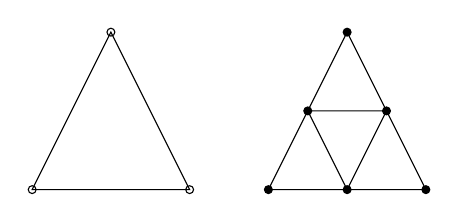
\begin{tikzpicture}
        % 三角形
        \draw (2, 1) -- (4, 1) -- (3, 3) -- cycle;
        % 三个顶点
        \draw (2, 1) circle(0.05cm);
        \draw (4, 1) circle(0.05cm);
        \draw (3, 3) circle(0.05cm);
        % 四个三角形
        \draw (5, 1) -- (6, 3) -- (7, 1) -- cycle;
        \draw (5.5, 2) -- (6.5, 2) -- (6, 1) -- cycle;
        % 六个顶点
        \draw [fill = black] (5, 1) circle(0.05cm);
        \draw [fill = black] (6, 3) circle(0.05cm);
        \draw [fill = black] (7, 1) circle(0.05cm);
        \draw [fill = black] (5.5, 2) circle(0.05cm);
        \draw [fill = black] (6.5, 2) circle(0.05cm);
        \draw [fill = black] (6, 1) circle(0.05cm);
      \end{tikzpicture}
      \caption{Left: pressure $p$ element, $\circ$ for degrees of $p$; 
               right: four velocity $v$ elements, $\bullet$ for degrees
               of $v$.}
      \label{fig::p-v}       
    \end{figure}
      
       The layout of the paper is arraged as follows. In section 2, we
    introduce the Navier-Stokes governing equations. In section 3, we
    illustrate data structure for finite element pair $4P1-P1$, In
    section 4, we use $4P1-P1$ elements to approximate the governing
    equations. Next in section 5, the AMG preconditioner for steady
    stokes equations is shown. In Section 6, we give the moving mesh
    strategy. Then we present numerical experiements in section 7. 
    Finaly, we give the conclusions in this section.

% ----------------------------------------------------------------------------------------
%	SECTION 3
% ----------------------------------------------------------------------------------------
    
\section{Governing Equation}

    Follow \cite{popiolek2006numerical} and \cite{elman2005finite}, we
    give nondimentional incompressible Navier-Stokes equations as
    follows:
    
    \begin{equation}
      \begin{array}{rcl}
         \partial_t \vec{u} - \nu \nabla^2 \vec{u} +
        (\vec{u} \cdot \nabla )\vec{u} + \nabla p & =
        & \vec{f},\\
        \nabla \cdot \vec{u} & = & 0,
      \end{array}
      \label{eq::NS}
    \end{equation}

    The vector $\vec{u}$ is velocity, and the scalar
    variable $p$ is pressure. The phisical domain $\Omega$ is in 2D or
    3D. The initial boundary value problem of the system
    (\ref{eq::NS}), with initial and boundary conditions on $\partial
    \Omega = \partial \Omega_D \bigcup \partial \Omega_N$:
    \begin{equation}
      \begin{array}{ll}
        \vec{u} = \vec{w},& \mbox{ on } \partial \Omega_D \times [0,
        T]\\
        \nu \displaystyle \frac{\partial \vec{u}}{\partial n} - p =
        \vec{0}, & \mbox{ on } \partial \Omega_N \times [0, T],  \\
        \vec{u}|_{t = 0} = \vec{u_0}, & \mbox{ in } \Omega. 
      \end{array}
      \label{eq::bc}
    \end{equation} 
    where $\vec{n}$ denotes the outward normal to the boundary. From
    equation (\ref{eq::bc}), we only need to give the value of
    preesure on $\Omega_N$. $\nu > 0$ is the constant kinematic
    viscosity.  

    Let $L$ represent a characteristic length scale for the domain
    $\Omega$. Let $U$ be the maximum value of velocity on the inflow,
    then the Reynolds number denotes:
    \begin{equation}
      Re := \frac{UL}{\nu}.
    \end{equation}
    
\section{Data Structure}
   In this paper finite element pair $4P1-P1$ is adopted. $4P1-P1$ is
   based on two different meshes and two different finite element
   spaces. Velocity mesh is obtained by globally refining pressure
   mesh. Mesh data structure is based on the hierarchy geometry tree
   in \cite{li2005multi}.
   \begin{figure}[h]
     \subfloat[One time uniform refined mesh]{
       \begin{minipage}[t]{0.4\textwidth}
         \centering
         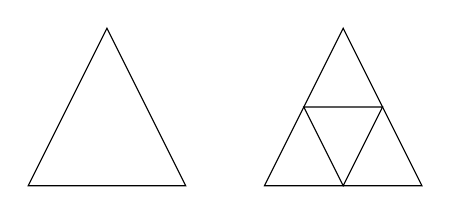
\begin{tikzpicture}
           % 三角形
           \draw (2, 1) -- (4, 1) -- (3, 3) -- cycle;
           \draw (5, 1) -- (6, 3) -- (7, 1) -- cycle;
           \draw (5.5, 2) -- (6.5, 2) -- (6, 1) -- cycle;
         \end{tikzpicture}
       \end{minipage}
     }
     \subfloat[its hierarchy tree]{
       \begin{minipage}[t]{0.6\textwidth}
         \centering
         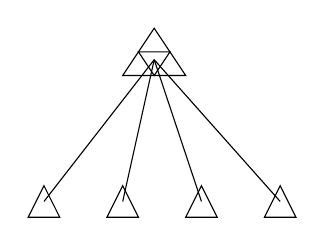
\begin{tikzpicture}
           %五个小三角形
           \draw (1.0, 0.0) -- (1.2, 0.4) -- (1.4, 0.0) -- cycle;
           \draw (2.0, 0.0) -- (2.2, 0.4) -- (2.4, 0.0) -- cycle;
           \draw (3.0, 0.0) -- (3.2, 0.4) -- (3.4, 0.0) -- cycle;
           \draw (4.0, 0.0) -- (4.2, 0.4) -- (4.4, 0.0) -- cycle;
           \draw (2.6, 2.4) -- (2.2, 1.8) -- (3.0, 1.8) -- cycle;
           \draw (2.4, 2.1) -- (2.6, 1.8) -- (2.8, 2.1) -- cycle;
           %四条线
           \draw (2.6, 2.0) -- (1.2, 0.2);
           \draw (2.6, 2.0) -- (2.2, 0.2);
           \draw (2.6, 2.0) -- (3.2, 0.2);
           \draw (2.6, 2.0) -- (4.2, 0.2);
         \end{tikzpicture}
       \end{minipage}
     }
     \caption{Hierachy tree structure}
     \label{fig::hgrometrytree}
   \end{figure}
   The four-fork tree is shown in Figure \ref{fig::hgrometrytree}.
   So a macro element(pressure) corresponds to four velocity elements. 
   By traversing all pressure elements one time, we can acquire the $1-1$
   index between elements of velocity and pressure based on the
   hierachy tree structure as algorithm \ref{alg::index} shown.  
   \begin{algorithm}
     \caption{Make index between velocity elements and pressure elements}
     \begin{algorithmic}[1]
       \State \text{achieveiterator} $\gets$ \text{irregualerMeshV.beginActiveElement()}
       \State \text{enditerator} $\gets$ \text{irregualerMeshV.endActiveElement()}
     
       \While {\text{achieveiterator} $\neq$ \text{enditerator}}
           \State \text{int index-v-element} $\gets$
                   \text{achieveiterator}$-\rangle$ \text{index}
           \State \text{HElement} $\langle$ \text{DIM,
                   DIM}$\rangle \ast$ \text{parent} $\gets$
                   \text{activeiterator}$-\rangle$ \text{parent}
           \State \text{int index-p-element} $\gets$
                   \text {parent}$-\rangle$ \text{index}
           \State \text{int n-child} $\gets$
                   \text{parent}$-\rangle$ \text{n-child}
           \State
                  \text{index-p2v[index-p-element].resize}(\text{n-child})
           \While {$i \geq 0$ \textbf{and} $i < \text{n-child}$}
                  \State \text{HElement}$\langle$\text{DIM,DIM}$\rangle$ $\ast$\text{chi}
                         $\gets$ \text{parent}$-\rangle$\text{child[i]}
                  \State \text{int index-v-element} $\gets$
                         \text{child}$-\rangle$\text{index}
                  \State \text{index-p2v[index-p-element][i]} $\gets$
                         \text{index-v-element}
                  \State \text{index-v2p[index-v-element]} $\gets$ \text{index-p-element}       
           \EndWhile
       \EndWhile
     \end{algorithmic}
     \label{alg::index}
   \end{algorithm}
   After the index built, we can assemble the element matrix for stiff
   matrix, mass matrix, and  divergence matrix for velocity and
   pressure only using P1 element.
\section{Finite Element Approximation}
    We define the solution and test spaces as
    \begin{eqnarray}
      \mathbf{H}_E^1 & := & \left\{ \vec{u} \in \mathcal{H}^1(\Omega)^d \big|
        \vec{u} = \vec{w} \mbox{ on } \partial \Omega_D \right\},\\
      \mathbf{H}_{E_0}^1 & := & \left\{ \vec{v} \in \mathcal{H}^1(\Omega)^d \big|
        \vec{u} = \vec{0} \mbox{ on } \partial \Omega_D \right\},
    \end{eqnarray}
    then the variational formulation is to find  $(\vec{u}, p) \in
   (\mathbf{H}_E^1, L_2(\Omega))$ such that
   \begin{eqnarray}
     \int_{\Omega}\frac{\partial \vec{u}}{\partial t} \cdot \vec{v} + 
     \nu \int_\Omega \nabla \vec{u} : \nabla \vec{v} + \int_\Omega \left(
       \vec{u} \cdot \nabla \vec{u} \right) \cdot \vec{v} - \int p
     \left( \nabla \cdot \vec{v} \right) & = & \int_\Omega \vec{f} \cdot
     \vec{v}, \label{eq::generalweak_momentum}\\
     & & \forall \vec{v} \in \mathbf{H}_{E_0}^1,\notag \\
     \int_\Omega q \left( \nabla \cdot \vec{u} \right) & = & 0,
     \label{eq::generalweak_mass} \\
     & & \forall q \in L_2(\Omega). \notag
   \end{eqnarray}
   Here $\nabla \vec{u} : \nabla \vec{v}$ represents the componentwise
   scalar product, $\nabla v_x \cdot \nabla u_x + \nabla
   v_y \cdot \nabla u_y$ in 2D.

   Assume $\tau_h$ is a triangulation of domain $\Omega$ for
   pressure mesh with mesh parameter $h = max_{T \in \tau_h} diam(T)$.
   While $\tau_{\frac{1}{2}h}$ is the triangulation for velocity mesh.
   Two finite element spaces $X_E^h$ and $P^h$ are seperatly based on
   $\tau_{\frac{1}{2}h}$ and $\tau_h$ such that
   \begin{equation}
     X_E^h \subset \mathcal{H}_E, \quad P^h \subset L_2(\Omega) 
     \notag 
   \end{equation}
   
   So (\ref{eq::generalweak_momentum}) and (\ref{eq::generalweak_mass})
    can be written as following : Find
   $(\vec{u}_h, p_h) \in X_E^h \times P^h$ such that
   \begin{equation}
     \begin{aligned}
       &\int_{\Omega}\frac{\partial \vec{u}_h}{\partial t} \cdot \vec{v}_h
       + \nu \int_\Omega \nabla \vec{u}_h : \nabla \vec{v}_h  \\
       + & \int_\Omega \left( \vec{u}_h \cdot \nabla \vec{u}_h \right)
       \cdot \vec{v}_h - \int_\Omega p_h \left( \nabla \cdot \vec{v}_h
       \right) & = &\int_\Omega \vec{f} \cdot \vec{v}_h, &\quad
       \forall \vec{v}_h \in \mathbf{X}_0^h;  \\
       & \int_\Omega q_h \left( \nabla \cdot \vec{u}_h \right) & = &0,&
       \quad \forall q_h \in P^h.
       \label{eq::discreted_weak}
     \end{aligned}
   \end{equation}

   Let $\{\phi_j \}_{j = 1}^n$ and $\{\psi_k\}_{k = 1}^m$ be linear basis
   functions for velocity and pressure. Nonlinear term $\vec{u}_h
   \cdot \nabla \vec{u}_h$ is explicitly treated. Then $u_h, v_h, p_h$
   can be written as follows.
   \begin{equation}
     u_h = \sum_{j = 1}^n u_j \phi_j, \quad v_h = \sum_{j = 1}^n v_j
     \phi_j, \quad p_h = \sum_{k = 1}^m p_k \psi_k 
     \notag
   \end{equation}
   Substituting the $u_h, v_h, p_h$ into (\ref{eq::discreted_weak}, 
   this obtains a linear system
   \begin{equation}
     \left[
       \begin{array}{lll}
         \frac{1}{dt} M + \nu A & 0 & B_x^T \\
         0 & \frac{1}{dt} M +\nu A  & B_y^T \\
         B_x & B_y & 0
       \end{array}
     \right]
     \left[
       \begin{array}{c}
          u_x \\
          u_y \\
          p
       \end{array}
     \right] = 
     \left[
       \begin{array}{c}
         f_x \\
         f_y \\
         g
       \end{array}
     \right],
     \label{eq::linear_system}
   \end{equation}
   Where the $n \times n$ matrix $M$ is the mass matrix and the Laplacian
   matrix is $A$, which are trivial.
   \begin{eqnarray}
     A = [a_{ij}], && a_{ij} = \int_\Omega \nabla \phi_i \cdot \nabla
     \phi_j \\
     M = [m_{ij}], && m_{ij} = \int_{\Omega}\phi_i \phi_j \\
   \end{eqnarray}
   the right hand side terms $f_x, f_y, g$ seperatly are
   \begin{eqnarray}
     f_x = [f_i], && f_i = \int_\Omega (\frac{u^{(n)}}{dt} - (u^{(n)}
       \frac{\partial u^{(n)}}{\partial x} + v^{(n)} \frac{\partial
       u^{(n)}}{\partial y}) \phi_i \notag \\
     f_y = [f_i], && f_i = \int_\Omega (\frac{u^{(n)}}{dt} - (u^{(n)}
       \frac{\partial v^{(n)}}{\partial x} + v^{(n)} \frac{\partial
         v^{(n)}}{\partial y}) \phi_i \notag \\
     g = [g_k], && g_i = 0. \notag
   \end{eqnarray}

    \begin{figure}
      \centering    
      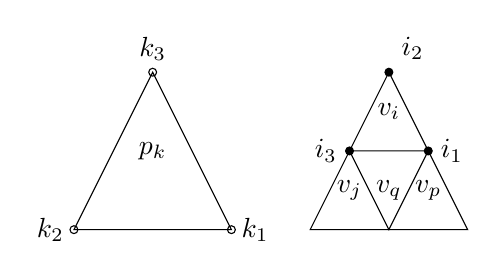
\begin{tikzpicture}
        % 三角形
        \draw (2, 1) -- (4, 1) -- (3, 3) -- cycle;
        % 三个顶点
        \draw (2, 1) circle(0.05cm);
        \draw (4, 1) circle(0.05cm);
        \draw (3, 3) circle(0.05cm);
        \draw (3, 2) node{$p_k$};
        % 三个顶点标号.
        \draw (1.7, 1) node {$k_2$};
        \draw (4.3, 1) node {$k_1$};
        \draw (3, 3.3) node {$k_3$};
        % 四个三角形
        \draw (5, 1) -- (6, 3) -- (7, 1) -- cycle;
        \draw (5.5, 2) -- (6.5, 2) -- (6, 1) -- cycle;
        % 六个顶点
        \draw [fill = black](6.5, 2) circle(0.05cm);
        \draw [fill = black](5.5, 2) circle(0.05cm);
        \draw [fill = black](6, 3) circle(0.05cm);
        % 三个顶点标号.
        \draw (6.8, 2) node {$i_1$};
        \draw (6.3, 3.3) node {$i_2$};
        \draw (5.2, 2) node {$i_3$};
        % 单元标记.
        \draw (6, 2.5) node {$v_i$};
        \draw (5.5, 1.5) node {$v_j$};
        \draw (6.5, 1.5) node {$v_p$};
        \draw (6, 1.5) node {$v_q$};
      \end{tikzpicture}
      \caption{Left: $p$ element; 
               right: four velocity $v$ elements corresponding to
               $p$ element by the index built last section.}
      \label{fig::matrix_assemble}       
    \end{figure}
   
   Here, we concentrate on the assembling of divergent matrix. Take 
   $B_x^T$ for instance. Let $\triangle_{v_i}$ be a velocity element,
   we can find the corresponding pressure element $\triangle_{p_k}$ 
   (see Figure \ref{fig::matrix_assemble}) by the index built last
   section. The local numbers of basis function is shown. $\phi_{i_1},
   \phi_{i_2}, \phi_{i_3}$ are the standard linear triangle basis
   functions defined on $\triangle_{v_i}$. While
   $\psi_{k_1}, \psi_{k_2}, \psi_{k_3}$ are defined on
   $\triangle_{p_k}$. Therefor, the element matrix of $B_x^T$ is 
   \begin{equation}
     \left[
     \begin{array}{lll}
       \int_{\triangle_{v_i}}\psi_{k_1} \frac{\partial
         \phi_{i_1}}{\partial x} & \int_{\triangle_{v_i}} \psi_{k_2}
       \frac{\partial \phi_{i_1}}{\partial x} & \int_{\triangle_{v_i}}
       \psi_{k_3} \frac{\partial \phi_{i_1}}{\partial x} \\
       \int_{\triangle_{v_i}} \psi_{k_1} \frac{\partial
         \phi_{i_2}}{\partial x} & \int_{\triangle_{v_i}} \psi_{k_2}
       \frac{\partial \phi_{i_2}}{\partial x} & \int_{\triangle_{v_i}}
       \psi_{k_3} \frac{\partial \phi_{i_2}}{\partial x} \\
       \int_{\triangle_{v_i}} \psi_{k_1} \frac{\partial
         \phi_{i_3}}{\partial x} & \int_{\triangle_{v_i}} \psi_{k_2}
       \frac{\partial \phi_{i_3}}{\partial x} & \int_{\triangle_{v_i}}
       \psi_{k_3} \frac{\partial \phi_{i_3}}{\partial x}
     \end{array}
   \right]
   \label{eq::element_matrix}
   \end{equation}
   
   Add the entries of element matrix to relavent position
   $(i_1,k_1)$, $(i_1, k_2)$, $(i_1, k_3)$, $(i_2, k_1)$, $(i_2, k_2)$,
   $(i_2,k_3)$, $(i_3, k_1)$, $(i_3, k_2)$, $(i_3, k_3)$ to  $B_x^T$. 
   After traversing all the velocity elements and adding element
   matrix (\ref{eq::element_matrix})to $B_x^T$, $B_x^T$ is completely
   assembled. Similarly, we can assemble matrix $B_y^T$.

   Conversly, by the index of pressure element $p_k$, we can find the 
   corresponding four small velocity elements $v_i, v_j, v_p, v_q$ see
   Figure \ref{fig::matrix_assemble}. After seperatly assembling the
   element $p_k$ with velocity elements $v_i, v_j, v_p, v_p$,  one
   pressure element matrix is built and add it to $B_x$. Repeat above 
   action until all the pressure elements are traversed. Therefor,
   $B_x$ is completely built. Assembling of $B_y$ is in the same way.    
   
   If we get rid of time term and nonlinear $\vec{u} \cdot \nabla
   \vec{u}$ in system (\ref{eq::NS}), we can get steady Stokes
   equations. After the same discretization, the linear sestem equation
   is as follows
   \begin{equation}
     \left[
       \begin{array}{lll}
         \nu A & 0 & B_x^T \\
         0 & \nu A  & B_y^T \\
         B_x & B_y & 0
       \end{array}
     \right]
     \left[
       \begin{array}{c}
          u_x \\
          u_y \\
          p
       \end{array}
     \right] = 
     \left[
       \begin{array}{c}
         \hat{f}_x \\
         \hat{f}_y \\
         \hat{g}
       \end{array}
     \right],
     \label{eq::linear_system_stokes}
   \end{equation}   
   The right hand side of (\ref{eq::linear_system_stokes}), we can set
   $\hat{f}_x = 0, \hat{f}_y = 0, \hat{g} = 0$ for simplicity.

   We solve the time-dependent Navier-Stokes system
   (\ref{eq::linear_system}) using GMRES method preconditioned with
   incomplete LU decomposition. In order to guarantee the numerical
   scheme stability, we choose the time adaptive step such that
   satisfing the CFL condition in each element. In order to illustrate
   our scheme, we demonstrate the flow-chart of the algorithm in
   (\ref{alg::solve}).

   \begin{algorithm}
     \caption{Moving mesh FEM for Navier Stokes equation}
     \begin{algorithmic}[1]
       \While {$t_n < T$}
             \State Solve Navier-Stokes
                    system(\ref{eq::linear_system}) in $t = t_n$ on the
                    velocity mesh $\triangle_v^{(n)}$ and pressure mesh
                    $\triangle_p^{(n)}$. Then obtain numerical solutions
                    $\vec{u}_h^{(n)}, p_h^{(n)}$.
             \State Caculate monitor function on $\triangle_p^{(n)}$
                    using $\vec{u}_h^{(n)}, p_h^{(n)}$. And obtain
                    logical mesh $\vec{\xi}^*$ by solving
                    (\ref{eq::logical}). \label{state::monitor}
             \State Judge if $L_2$ norm of $\vec{\xi}^* -
                    \vec{\xi}^{(0)}$ is less than tolerance. If yes,
                    the iterator is over. Else, continue
                    \ref{state::start} - \ref{state::end}.
             \State Caculate move direction $\delta \vec{x}$ of
                    $\triangle_p^{(n)}$ using the difference of
                    $\vec{\xi}^* - \vec{\xi}^{(0)}$. 
                    \label{state::start}
             \State Solve equation (\ref{eq::continous_update}) on
                    $\triangle_v^{(n)}$ to get medium variable 
                    $\vec{u}_{h, *}^{(n)}, p_{h, *}^{(n)}$ on new
                    mesh.
             \State Update $\triangle_p^{(n)}$ to $\triangle_p^{(n + 1)}$, Sync
                    $\triangle_v^{(n)}$ by the hierachy geometry tree
                    stucture to $\triangle_v^{(n + 1)}$.
             \State Go back to \ref{state::monitor}. \label{state::end}       
             
             \State Solve Navier-Stokes system
                    (\ref{eq::linear_system}) to truely obtain numerical
                    solutions $\vec{u}_h^{(n + 1)}, p_h^{(n + 1)}$ on
                    mesh $\triangle_v^{(n + 1)}$ and $\triangle_p^{(n
                      + 1)}$.
        \EndWhile     
     \end{algorithmic}
     \label{alg::solve}
   \end{algorithm}
   
   \section{Precondition strategy}
   
   \subsection{AMG precondition for steady stokes equations}
   
   For simplicity, we choose the steady Stokes equations to show
   efficiency of AMG preconditioner. Recall linear system
   (\ref{eq::linear_system_stokes}), which is indedinite, we choose a
   Krylov subspace method, MINRES as the solver. As we known, to make 
   sure the efficency of MINRES, we should choose an efficient
   preconditioner. Motivated by the work in \cite{elman2005finite},
   pressure mass matrix $Q$ can be an approximation of the schur
   complement of coefficient matrix in
   (\ref{eq::linear_system_stokes}) and $\hat{Q} = diag(Q)$ works well
   in practical computation.  Here, we choose matrix K
   \begin{equation}
     K = \left[
           \begin{array}{lll}
             \nu A & 0 & 0 \\
             0 & \nu A  & 0 \\
             0 & 0 & \hat{Q}
           \end{array}
         \right]     
   \end{equation}
   as an approximation to the coefficient matrix M 
   \begin{equation}
     M = \left[
           \begin{array}{lll}
             \nu A & 0 & B_x^T \\
             0 & \nu A  & B_y^T \\
             B_x & B_y & 0
           \end{array}
         \right],     
   \end{equation}
   In precondition, we often need to apply the action of $K^{-1}$.
   Instead of solving $V_{des} = K^{-1} V_{src}$, we use an AMG
   solver (for $P1$ element) of AFEPack(a finite element package) to
   solve block $(0, 0)$ and $(1, 1)$ of system $K V_{des} = V_{src}$, 
   where $V_{src}$ is given and $V_{des}$ is unknown. AFEPack can be
   obtained from \url{http://dsec.pku.edu.cn/~rli}.
   
\section{Moving mesh  Stategy}
   At time $t = t_{n + 1}$, by scheme mentioned above, we can get
   numerical solutions $\vec{u}_h^{(n + 1)}, p_h^{(n + 1)}$ on old
   mesh $\mathcal{T}_h^n$. We follow the framework in
   \cite{di2005moving} to implement divergence-free
   interpolation of $(\vec{u}_h^{(n + 1)}, p_h^{(n + 1)})$ from
   $\mathcal{T}_h^n$ to new mesh $\mathcal{T}_h^{(n + 1)}$.
   Noticing that common Dirichlet and Neumann boundary
   condition are considered instead of periodic boundary condition.
   Briefly speaking, the moving mesh strategy mainly contains four
   steps as follows.
   \subsection{Step 1 Obtain monitor function}
      Choices of an appropriate monitor function are very important for
      adaptive scheme. Let $m = 1/G$, where $G$ is the monitor
      function. As illustrated in \cite{di2005moving}, there are some
      common choices of $G$. One based on vorticity is 
      \begin{equation}
        \centering
        G_0 = \sqrt{1 + \alpha |\omega|^\beta}.
        \label{eq::monitor_vorticity}
      \end{equation}
      where $\omega = \nabla \times \vec{u}$, $\alpha, \beta$
      are positive constants. It is illustrated in \cite{cao1999anr}
      that $\beta = 4$ is a good choice for adaptation in flow past
      cylinder problem. In this work, $\alpha = 0.5, \beta = 2$ shows
      good result. Another selection of $G$ is demonstrated as
      follows, which based on the gradient of solution.
      \begin{equation}
        G_1(\vec{u}) = \sqrt{1 + \alpha |\nabla \vec{u}|^\beta}
        \label{eq::monitor_gradient}
      \end{equation}
      where $\vec{u}$ is velocity variable. This monitor function is
      used for problems which solutions have large gradients, such as
      colliding flow which are used for accuracy test for our
      algorithm.
   \subsection{Step 2 Get a new logical mesh}
      In \cite{li2001mesh}, by solving elliptic equation 
      \begin{equation}
        \nabla_{\vec{x}}(m \nabla_{\vec{x}} \vec{\xi}) = 0
        \label{eq::logical}
      \end{equation}
      with Dirichlet boundary condition 
      \begin{equation}
        \vec{\xi}|_{\partial \Omega} = \vec{\xi}_b
        \label{eq::EL_boundary}
      \end{equation}
      a new logical mesh $\mathcal{T}_c^*$ with its nodes
      $\mathcal{A}^*$ is obtained.

   \subsection{Step 3 Achieve mesh move direction in physical domain}
      Several notaions are introduced firstly. $\mathcal{T}_h$ is the
      triangulation of physical domain, and its i th node denotes $X_i$. 
      Meantime, $T_i$ is the set of elements containing $X_i$.
      Correspondingly, on the logical domain the notations are
      $\mathcal{T}_c, \mathcal{A}_i, T_{i, c}$. $(\mathcal{A}_i^1,
      \mathcal{A}_i^2)$ are denoted as the coordinates of i th node
      $\mathcal{A}_i$ in the logical domain. According to Step 1 and
      Step 2, a new logical mesh $\mathcal{T}_c^*$ is got, meanwhile
      $\mathcal{A}_i^*$ is its $i$ th node. Therefore we can attain the
      error of $i$ th node:
      \begin{equation}
        \delta \mathcal{A}_i = \mathcal{A}_i^0 - \mathcal{A}_i^*
      \end{equation}
      where $\mathcal{A}_i^0$ is the $i$th node of the initial logical
      mesh $\mathcal{T}_c^0$. To be noticed that once the initial
      logical mesh is obtained, it maintains unchange until the whole
      algorithm is over.
      
      For a given element $E$ in $\mathcal{T}_h$, its vertexes are
      denoted as $X_k, 0 \leq k \leq 2$. Piecewise linear map from
      $V_{T_c^*}(\Omega_c)$ to $V_T(\Omega)$ has constant gradient 
      $\partial \vec{x} / \partial \xi $ on E, which can be obtained by 
      solving following system
      \begin{eqnarray}
        \begin{aligned}
          & \left (
            \begin{array}{cc}
              \mathcal{A}_{E_1}^{*, 1} - \mathcal{A}_{E_0}^{*, 1} & 
              \mathcal{A}_{E_2}^{*, 1} - \mathcal{A}_{E_0}^{*, 1} \\
              \mathcal{A}_{E_1}^{*, 2} - \mathcal{A}_{E_0}^{*, 2} &
              \mathcal{A}_{E_2}^{*, 2} - \mathcal{A}_{E_0}^{*, 2} 
            \end{array} 
          \right )
          \left (
            \begin{array}{cc}
              \frac{\partial x^1}{\partial \xi^1} & \frac{\partial
                x^1}{\partial \xi^2} \\
              \frac{\partial x^2}{\partial
                \xi^1} & \frac{\partial x^2}{\partial \xi^2}
            \end{array}
          \right ) \notag \\ = & 
          \left (
            \begin{array}{ll}
              X_{E_1}^1 - X_{E_0}^1 & X_{E_2}^1 - X_{E_0}^1 \\
              X_{E_1}^2 - X_{E_0}^2 & X_{E_2}^2 - X_{E_0}^2 
            \end{array}
          \right )
        \end{aligned}
      \end{eqnarray}
      If we let the volume of the element as the weight, the weighted 
      average displacement of the $i$th node $X_i$ is as follows:
      \begin{eqnarray}
        \delta X_i = \frac{\sum\limits_{E \in T_i} |E| \frac{\partial
            \vec{x}}{\partial \xi}|_{\text{in} E} \delta
          \mathcal{A}_i}{\sum\limits_{E \in T_i} |E|}.
      \end{eqnarray}
      where $|E|$ is the volume of element $E$.
      We also choose a positive parameter $\mu$ to prevent mesh
      tangling. Assume that the new mesh on the physical domain is
      denoted as $\mathcal{T}^*$, and its nodes $X_i^*$
      \begin{equation}
        X_i^* = X_i + \mu \delta X_i
      \end{equation}
      The method of selecting $\mu$ see \cite{di2005moving} for detail. 
   \subsection{Step 4 Eusure the incompressible constraint
     interpolation}
      It is required to maintain divergence-free in the interpolation
      when implementing moving mesh method to solving incompressible
      flow. In \cite{di2005moving}, solution re-distribution on the new 
      mesh $\mathcal{T}^*$ is achieved by solving lineard inviscid 
      Navier-Stokes-type equations.
      \begin{eqnarray}
        \frac{\partial \vec{u}}{\partial \tau} - \nabla_{\vec{x}}\vec{u}
        \cdot \delta \vec{x} & = & - \nabla p. \\
        \nabla_{\vec{x}}\cdot \vec{u} & = & 0
        \label{eq::continous_update}
      \end{eqnarray} 
      where $\delta \vec{x} := x^{\text{old}} - x^{\text{new}}$,
      $x^{\text{old}}, x^{\text{new}}$ are two sets of coordinates in
      physical domain. $\tau$ is a virtual time variable and often
      choosen as $1$. Here $p$ is just an intermediate variable,
      different from pressure variable in (\ref{eq::NS}). 

      Weak form of (\ref{eq::continous_update}) is : find $(\vec{u}_h,
      p_h) \in X_E^h \times P^h$ such that 
      \begin{eqnarray}
        \begin{aligned}
          \left( \partial_{\tau} \vec{u}_h - \nabla_{\vec{x}}\vec{u}_h
            \cdot \delta \vec{x}, \vec{v}_h \right) & = & \left( p_h, \nabla
            \vec{v}_h \right). \quad \forall \vec{v}_h \in X_E^h \\
          \left( \nabla_{\vec{x}} \cdot \vec{u}, q_h\right) & = & 0. \quad \forall
          q_h \in P^h
        \end{aligned}
        \label{eq::discreted_update}
      \end{eqnarray}
      
      In this work, we apply full implicity scheme which is
      unconditional stable, instead of
      three-step Runge-Kutta in \cite{di2005moving}, to
      (\ref{eq::discreted_update}) for time discretization:
      \begin{eqnarray}
        \begin{aligned}
          \left ( \frac{u_{h, *}^{(n)} - u_h^{(n)}}{\triangle \tau},
            \vec{v}_h \right) + \left( \delta \vec{x} \cdot \nabla 
            \vec{u}_{h, *}^{(n)}, \vec{v}_h \right)  & = & \left( 
            p_{h, *}^{(n)}, \nabla \vec{v}_h \right) \\
          \left( \nabla \cdot u_{h, *}^{n}, q_h \right) & = & 0.
        \end{aligned}
      \end{eqnarray}
      where $\vec{u}_h^{(n)}$ and $p_h^{(n)}$ are the numerical solutions of
      Navier-Stokes equations at $t = t_{n + 1}$ using the mesh at $t
      = t_n$. $u_{h,*}^{(n)}$ and $p_{h, *}^{(n)}$ are the intermediate
      updated solutions at $t =t_{n + 1}$ on the new mesh. 
   
\section{Numerical Tests}
     There are three numerical tests here. In practical computing, 
     we use solutions of Stokes equations as initial value of
     Navier-Stokes equations.  We show moving mesh and numerical
     solutions in the following. Our codes are based on the AFEPack.

     \subsection{Jetting flow into a static field}
       This example models a thin flow jetting into a channel with
       static flow field.  
       Our computional domain is $\Omega = [0, 12] \times [-3, 3]$ and
       viscosity is $\nu = 0.0005$.
       Natural outflow boundary is imposed on $x = 12$, while inflow
       boundary condition $u_x = 1 - 100 y^2, u_y = 0$ on $x = 0, y
       \in [-0.1, 0.1]$. No-slip boundary condition is setted on
       other boundary of $\Omega$. 
       
       We select (\ref{eq::monitor_vorticity}) as monitor in our
       moving strategy. Parameters $\alpha = 2.0, \beta = 2.0$ perform
       well. As we known, when a thin flow jets into static
       field, two symmetric vortexes appears along the jetting flow.
       For improving the computional precision, it requires more grids
       around the flow. From Figure \ref{fig::jetting_flow_mesht12s}, mesh 
       is concentrated around the vorticity contour with large
       velocity gradient. As time evolving, fluid instability will apper as
       Figure \ref{fig::jetting_flow_mesht27s} shown which is
       consistent with phisical phenomena.

       \begin{figure}[!htbp]
         \begin{center}
%             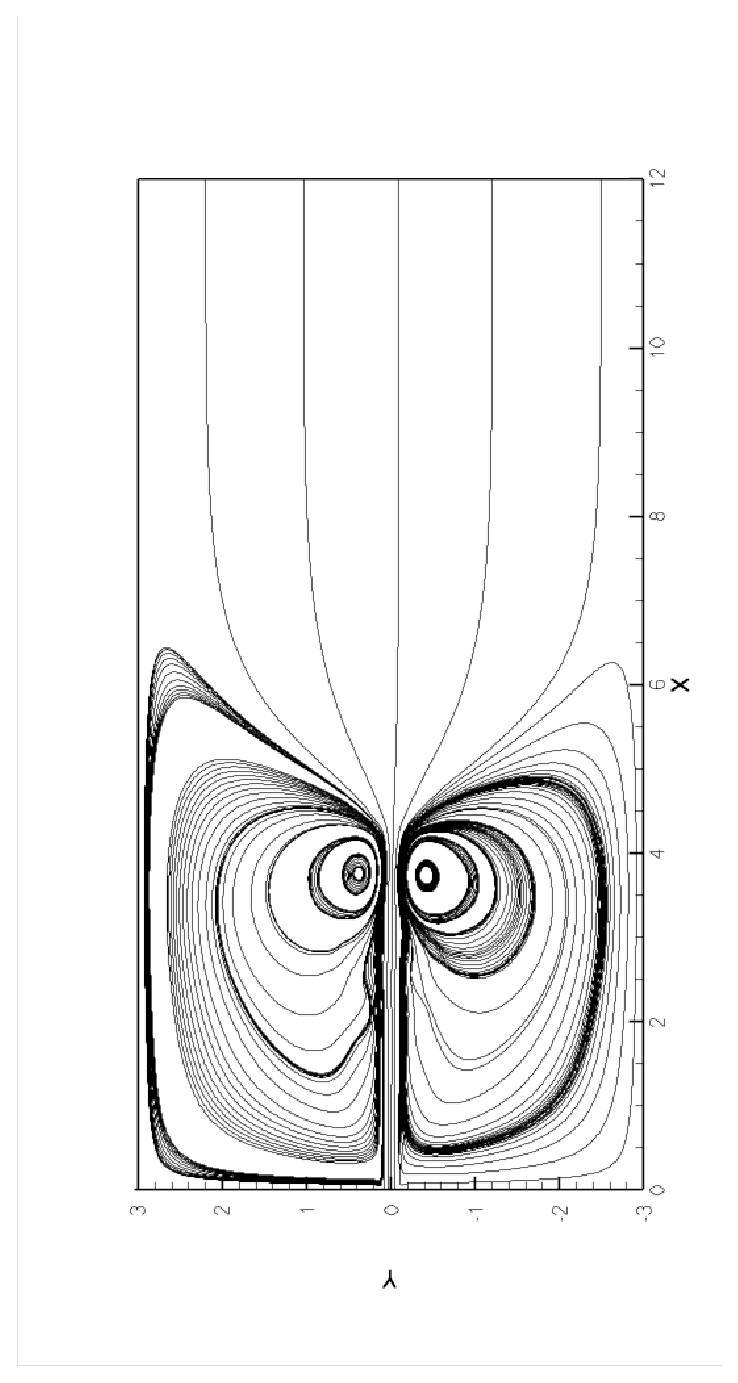
\includegraphics[width = 0.53\textwidth, angle = -90]{picture/jet_flow_data/streamline_t12s.eps}
             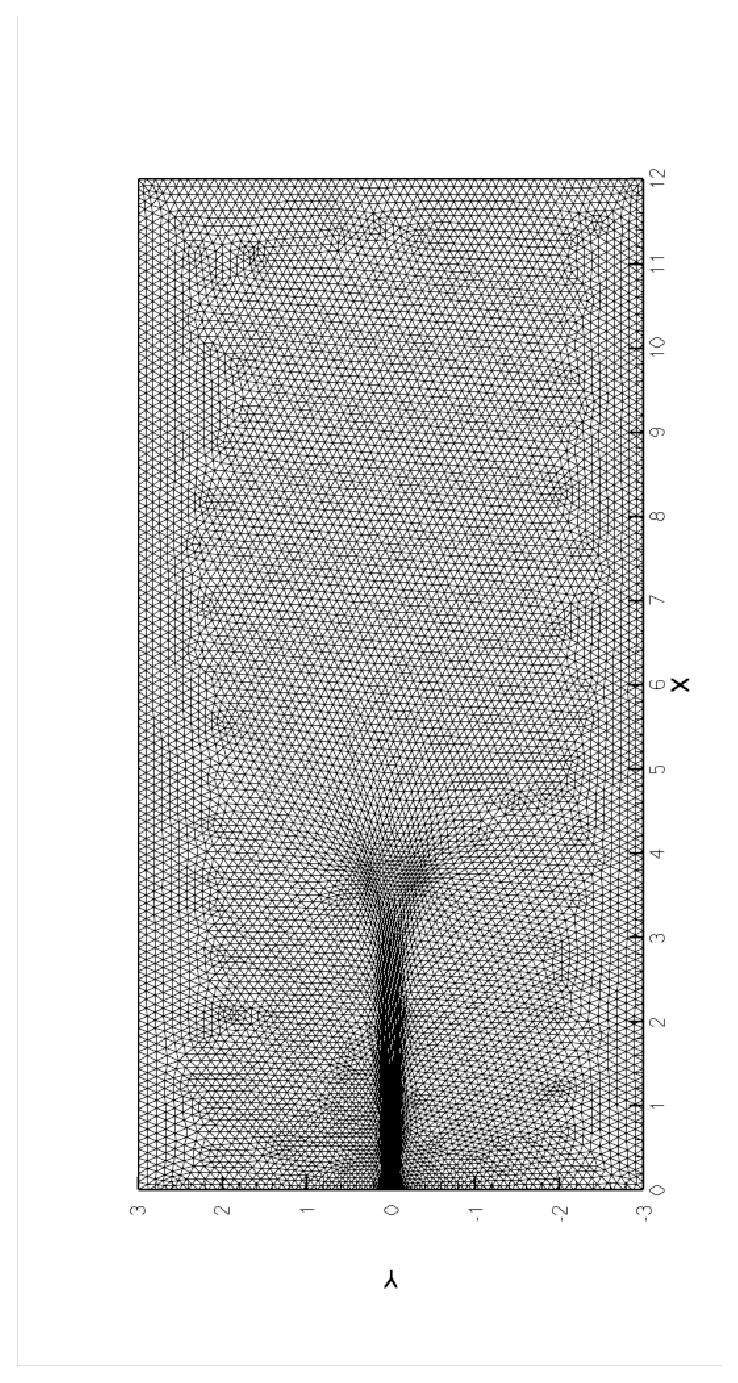
\includegraphics[width = 0.53\textwidth, angle = -90]{picture/jet_flow_data/mesh_t12s.eps}
             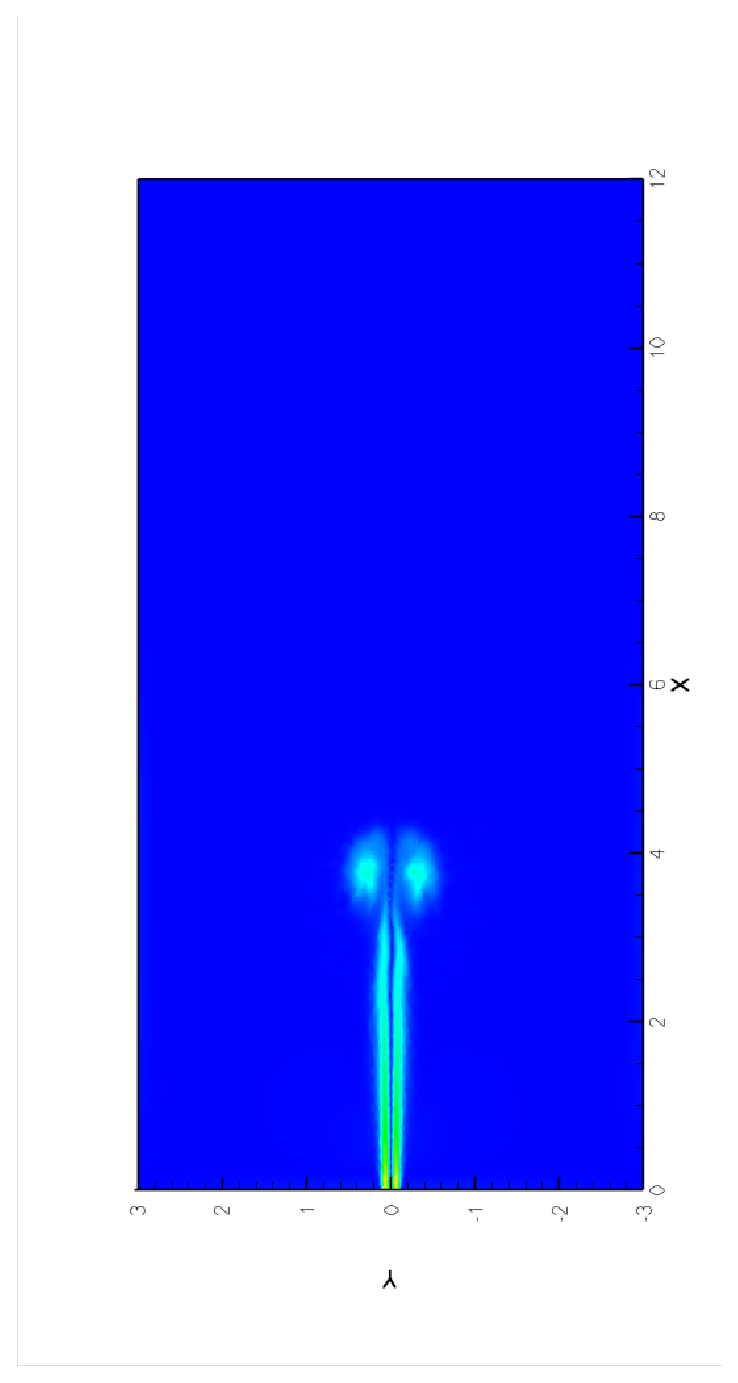
\includegraphics[width = 0.53\textwidth, angle = -90]{picture/jet_flow_data/contour_t12s.eps}
        \end{center}
        \caption{\small Jetting flow: top: mesh, bottom: vorticity contour at t = 12s.}
        \label{fig::jetting_flow_mesht12s}
       \end{figure}

       \begin{figure}[!htbp]
         \begin{center}
             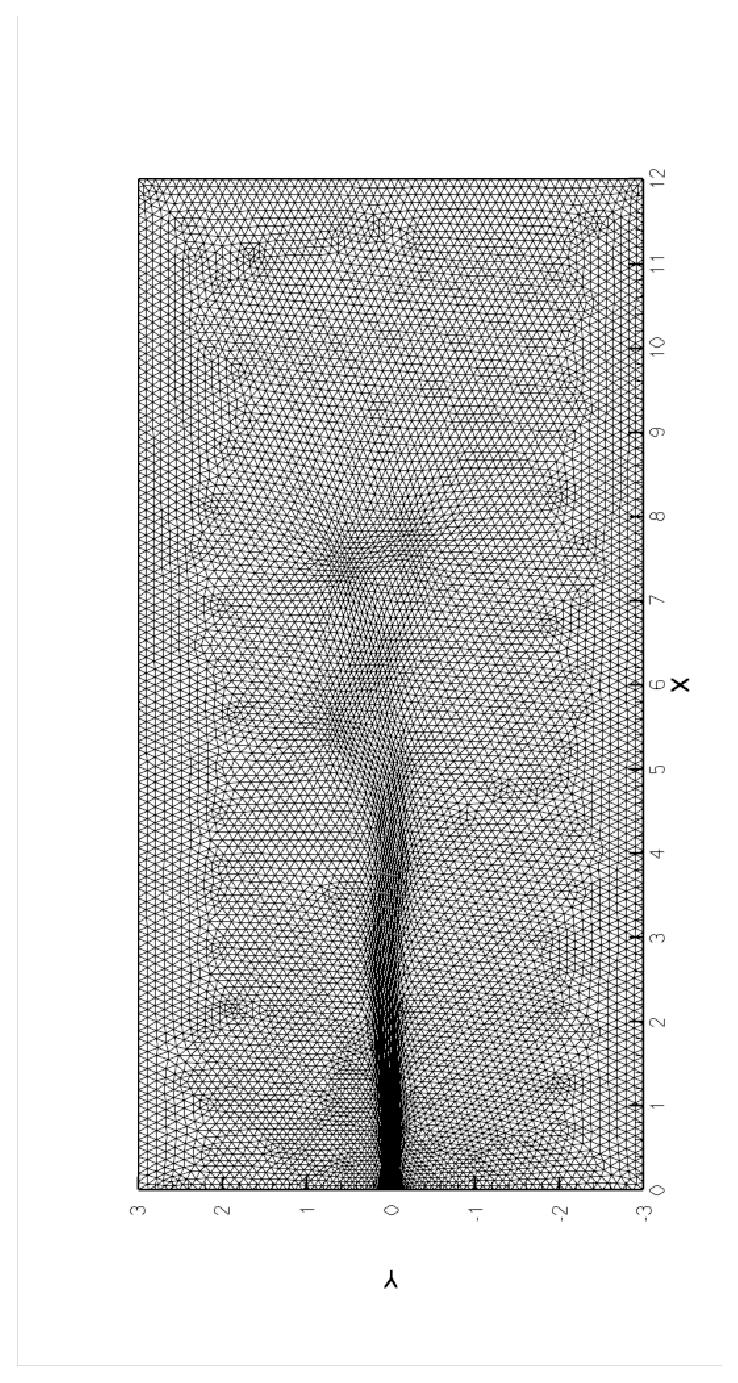
\includegraphics[width = 0.53\textwidth, angle = -90]{picture/jet_flow_data/mesh_t27s.eps}
             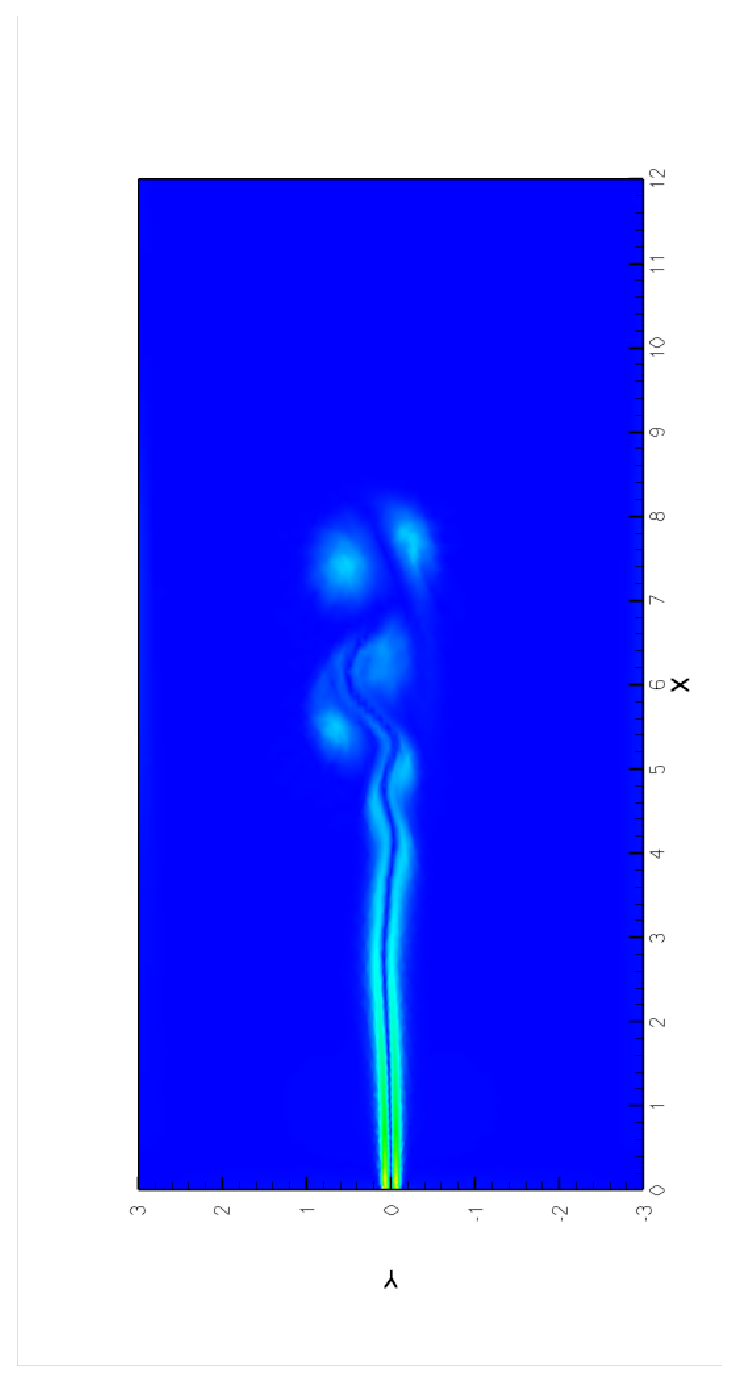
\includegraphics[width = 0.53\textwidth, angle = -90]{picture/jet_flow_data/contour_t27s.eps}
        \end{center}
        \caption{\small Jetting flow: top: mesh, bottom: vorticity contour at t = 27s.}
        \label{fig::jetting_flow_mesht27s}
       \end{figure}
       
       
     % \subsection{Colliding Flow}    
     %    This test problem has analytic solutions for steady Stokes system
     %    (\ref{eq::linear_system_stokes}) with $\nu = 1.0$ as follows:
     %    \begin{equation}
     %      u_x = 20 x y^3; \quad u_y = 5 x^4 - 5 y^4; \quad p = 60 x^2 y - 20
     %      y^3 + \mbox{constant}.
     %      \label{eq::colliding}
     %    \end{equation}
        
     %    This example is used to check the accuracy of our moving mesh
     %    algorithm. As we known error estimates in
     %    \cite{bercovier1979error}: velocity has second-order
     %    convergent rate, while pressure first-order. We expect that
     %    our moving mesh algorithm has the same convergent rate. In
     %    this test problem, we choose monitor
     %    (\ref{eq::monitor_gradient}) based on gradient, and the
     %    parameter $\alpha = 0.005, \beta = 2$. 
        
     %    From Table \ref{tab::colliding_moving_error}, we can
     %    conclude that $||\vec{u} - \vec{u}_h||_{L^2}$ decreases by one-fouth with
     %    successive uniform refinement. It is consistent with the error bound
     %    for velocity in \cite{bercovier1979error}. While the
     %    convergence order of $||p - p_h||_{0, \Omega}$ is more than
     %    one. The $l_2$ error of the numerical vorticity and divergence
     %    are listed in Table
     %    (\ref{tab::colliding_moving_div_error}). It is observed that a
     %    first-order convergence rate for vorticity and divergence.

     %    In Figure \ref{fig::colliding_flow_mesh}, the pressure
     %    contour, velocity streamline and moving mesh are shown. The
     %    mesh is different from the uniform mesh. Mesh is clustered to
     %    four corners for large gradient of velocity solutions in the
     %    corner.

     %    From Table \ref{tab::colliding_uni_refine},
     %    it can be seen that the iterative steps of MINRES in solving linear
     %    system (\ref{eq::linear_system_stokes}) is independent of
     %    total degree of freedom. 


     %    \begin{table}[!htbp]
     %      \centering
     %      \begin{tabular}{ccc} \toprule
     %        total $n_{\text{dof}}$   &\multicolumn{2}{c} {steps of
     %          MINRES} \\ \midrule 
     %                 &    AMG     &  without AMG \\  
     %        1183     &    91      &   867          \\  
     %        4523     &    97      &   1938         \\  
     %        17683    &    96      &   4106         \\
     %        69923    &    94      &   8415       \\
     %        278083   &    92      &   16866      \\
     %        1109123  &    91      &   -----       \\
     %        \bottomrule
     %      \end{tabular}
     %      \caption{\small Colliding flow: solving with AMG precondition, $\nu
     %        = 1.0$.}
     %      \label{tab::colliding_uni_refine}
     %    \end{table}

     %      \begin{table}[!htbp]
     %        \centering
     %        \begin{tabular}{ccccccc} \toprule
     %          mesh   & $||\vec{u} - \vec{u}_h ||_{L^2}$ & order&$||\vec{u} -
     %          \vec{u}_h ||_{H^1}$ & $||p - p_h||_{L^0}$ & order &$||p -
     %          p_h||_{H^1}$  \\ \midrule
     %          $10 \times 10$   &   $1.15 \times 10^{-1}$   &  &  $3.22 \times
     %          10^0$     &   $7.74 \times 10^{-1}$ & & $1.82 \times 10^1$    \\  
     %          $20 \times 20 $   &   $2.96 \times 10^{-2}$   & 1.94  &  $1.62 \times
     %          10^0$     &   $2.09 \times 10^{-1}$ & 1.99 & $1.05 \times 10^1$   \\
     %          $40 \times 40 $   &   $7.48 \times 10^{-3}$   & 1.98  & $8.12 \times
     %          10^{-1}$  &   $5.96 \times 10^{-2}$ & 1.75 & $5.99
     %          \times 10^0$   \\ \bottomrule
     %        \end{tabular}
     %        \caption{\small Colliding flow: accuracy test for the moving mesh velocity
     %          and pressure solution, $\nu = 1.0$.}
     %        \label{tab::colliding_moving_error}
     %      \end{table}

     %      \begin{table}[!htbp]
     %        \centering
     %        \begin{tabular}{ccccc} \toprule
     %          mesh   & vorticity $L^2$ error & order & divergence
     %          $L^2$ error & order\\ \midrule
     %          $10 \times 10$    &   $2.18 \times 10^{0}$   &  &   $2.36 \times
     %          10^0$ &  \\
     %          $20 \times 20 $   &   $1.09 \times 10^{0}$  & 1.00 &   $1.19 \times
     %          10^0$ & 0.99 \\
     %          $40 \times 40 $   &   $5.46 \times 10^{-1}$ & 1.00 &   $6.01 \times
     %          10^{-1}$ &  0.99 \\ \bottomrule
     %        \end{tabular}
     %        \caption{\small Colliding flow: accuracy test for
     %          divergence and vorticity, $\nu = 1.0$.}

     %        \label{tab::colliding_moving_div_error}
     %      \end{table}

     %      \begin{figure}[!htbp]
     %        \begin{center}
     %          \begin{minipage}{0.495\textwidth}
     %            \centering
     %            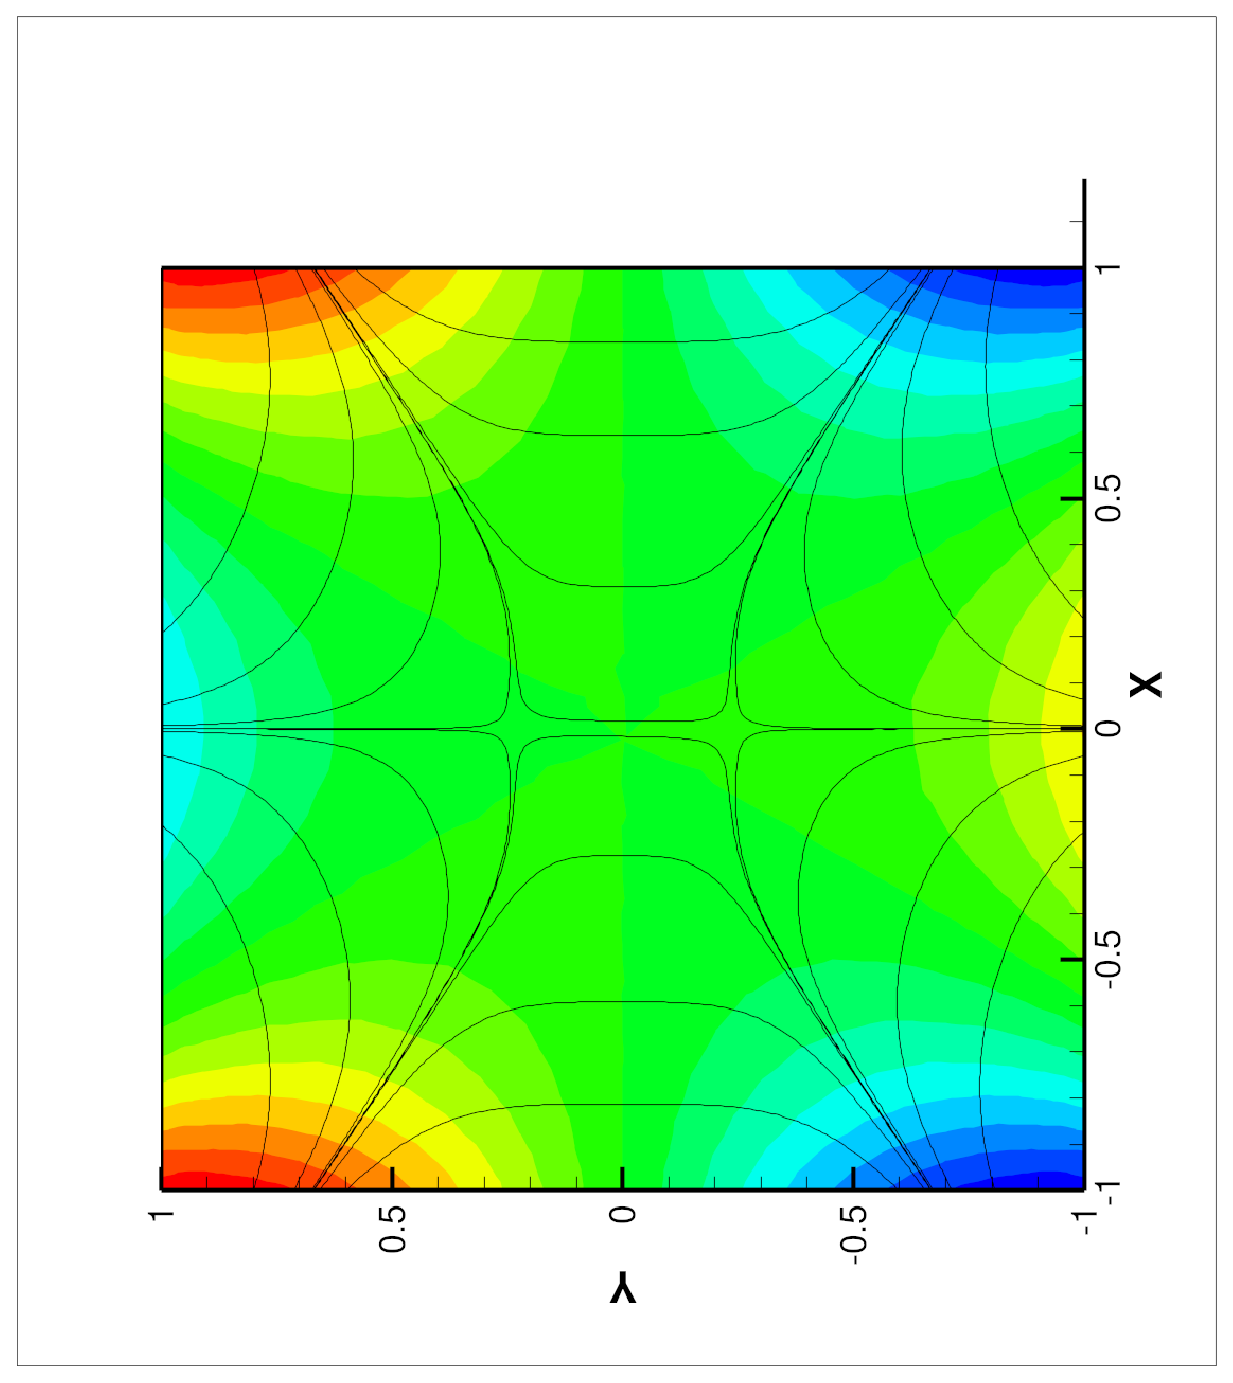
\includegraphics[width = 1.0\textwidth, angle =
     %            -90]{picture/colliding_flow_data/streamline_20_005.eps}
     %          \end{minipage}
     %          \begin{minipage}{0.495\textwidth}
     %            \centering
     %            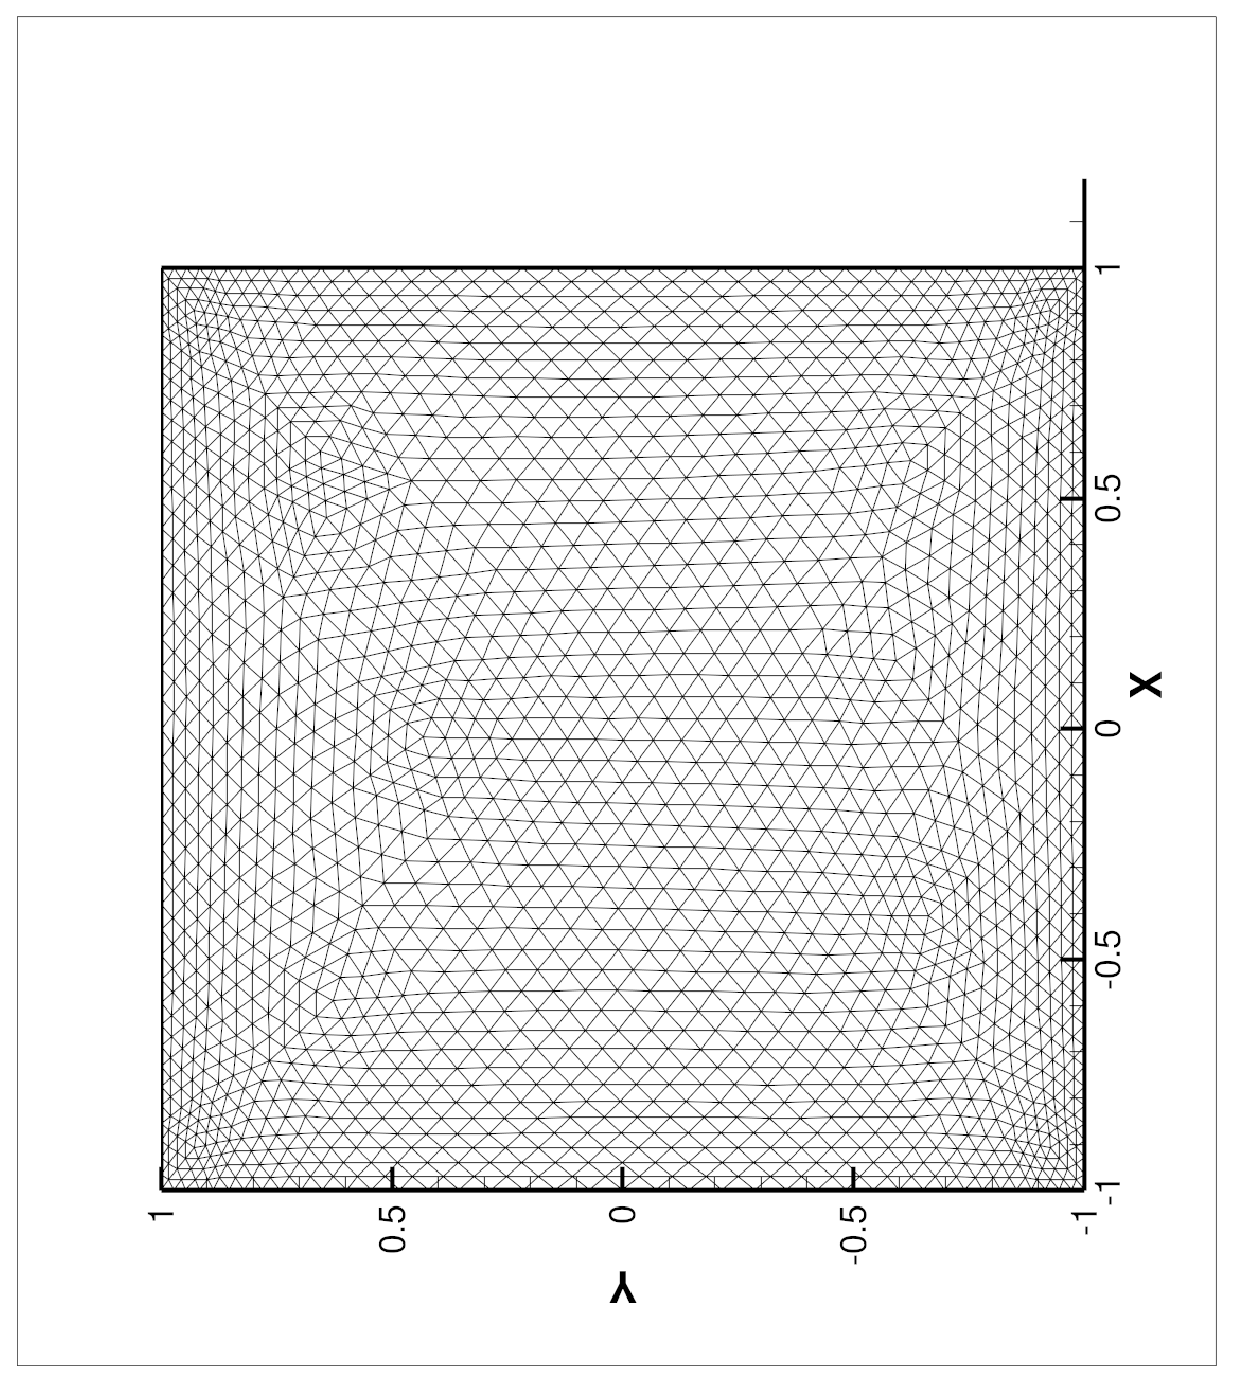
\includegraphics[width = 1.0\textwidth, angle = -90]{picture/colliding_flow_data/mesh20_005.eps}
     %          \end{minipage} 
     %          \caption{\small Colliding flow: left: velocity streamline and pressure contour; right: mesh.}
     %          \label{fig::colliding_flow_mesh}
     %        \end{center}
     %      \end{figure}

   \subsection{Navier-Stokes flow over a step}

      We consider the test problem in \cite{zheng2010posteriori} that the
      Navier-Stokes flow over a step with $\text{Re} = 1000$. The
      domain is $\Omega = (0, 4) \times (0, 1)/(1.2, 1.6) \times (0,
      0.4)$, and on the upper and bottom boudaries, Dirichlet
      condition $\vec{u} = (0, 0)^T$ is imposed. Outflow boundary is
      enforced natural boundary condition meanwhile at the inflow
      boundary $\vec{u} = (4 y (1 - y), 0)$.

      (\ref{eq::monitor_vorticity}) is selected as monitor function
      based on vorticity with $\alpha = 0.4, \beta = 2.0$. As we
      known, singularities arise at the concave corner in this
      problem. Figure \ref{fig::step_initial_mesh} shows the initial
      moving mesh clusters near the concave edge. Figure
      \ref{fig::step_flow_05s}, \ref{fig::step_flow_1s} and
      \ref{fig::step_flow_2s} show moving mesh and contour of
      vorticity at $t = 0.5s, t = 1s \text{, and } t = 2s$. It is
      observed that our moving mesh is consistent with the structure of
      vorticity.

      Pressure contour and velocity streamline at $t = 2s$ are shown
      in Figure \ref{fig::step_flow_contour_streamline_2s}.      
       
      \begin{figure}[!htbp]
        \begin{center}
        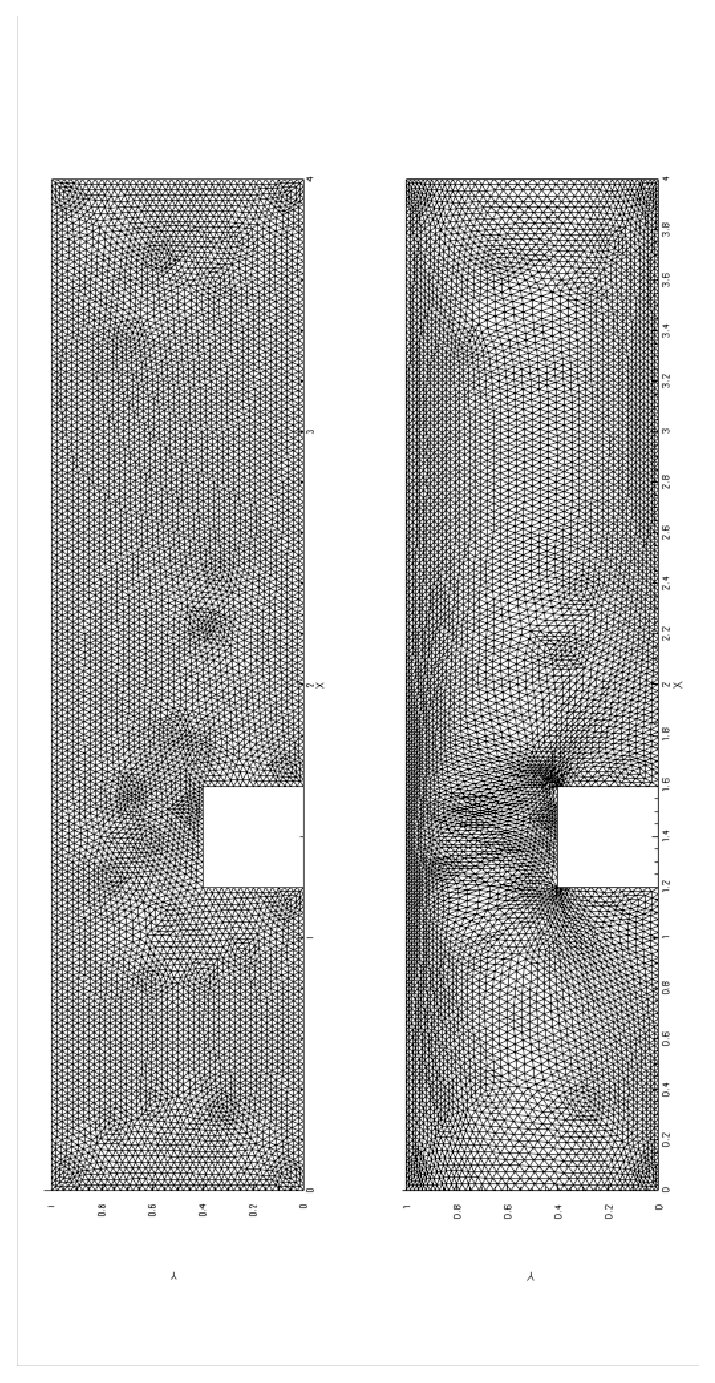
\includegraphics[width = 0.55\textwidth, angle = -90]{picture/step_flow_data/initial_mesh40_001.eps}
        \caption{\small Up: Initial uniform mesh; bottom: initial moving mesh.}
        \label{fig::step_initial_mesh}
        \end{center}
      \end{figure}

      \begin{figure}[!htbp]
        \centering
        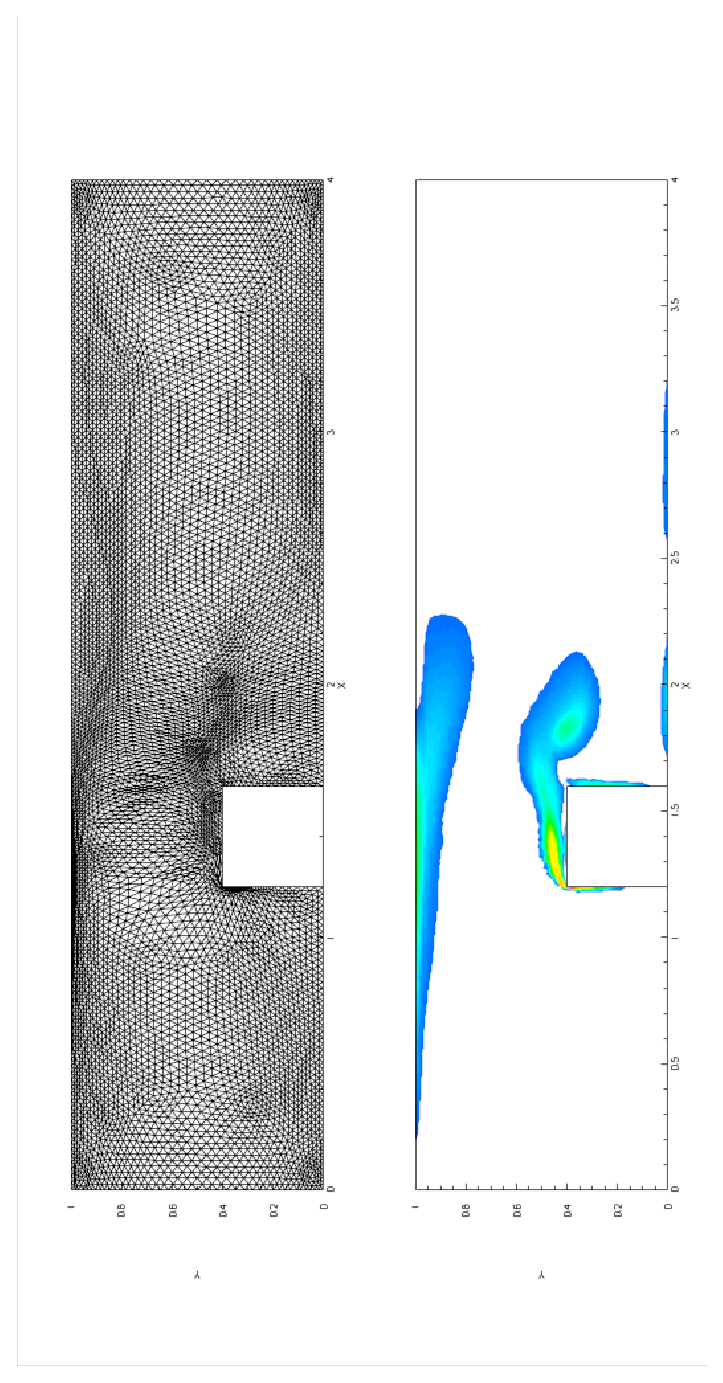
\includegraphics[width = 0.55\textwidth, angle = -90]{picture/step_flow_data/mesh_t_05.eps}
        \caption{\small Up: moving mesh; bottom: contour of vorticity
          at t = 0.5s}
        \label{fig::step_flow_05s}
      \end{figure}

      \begin{figure}[!htbp]
        \centering
        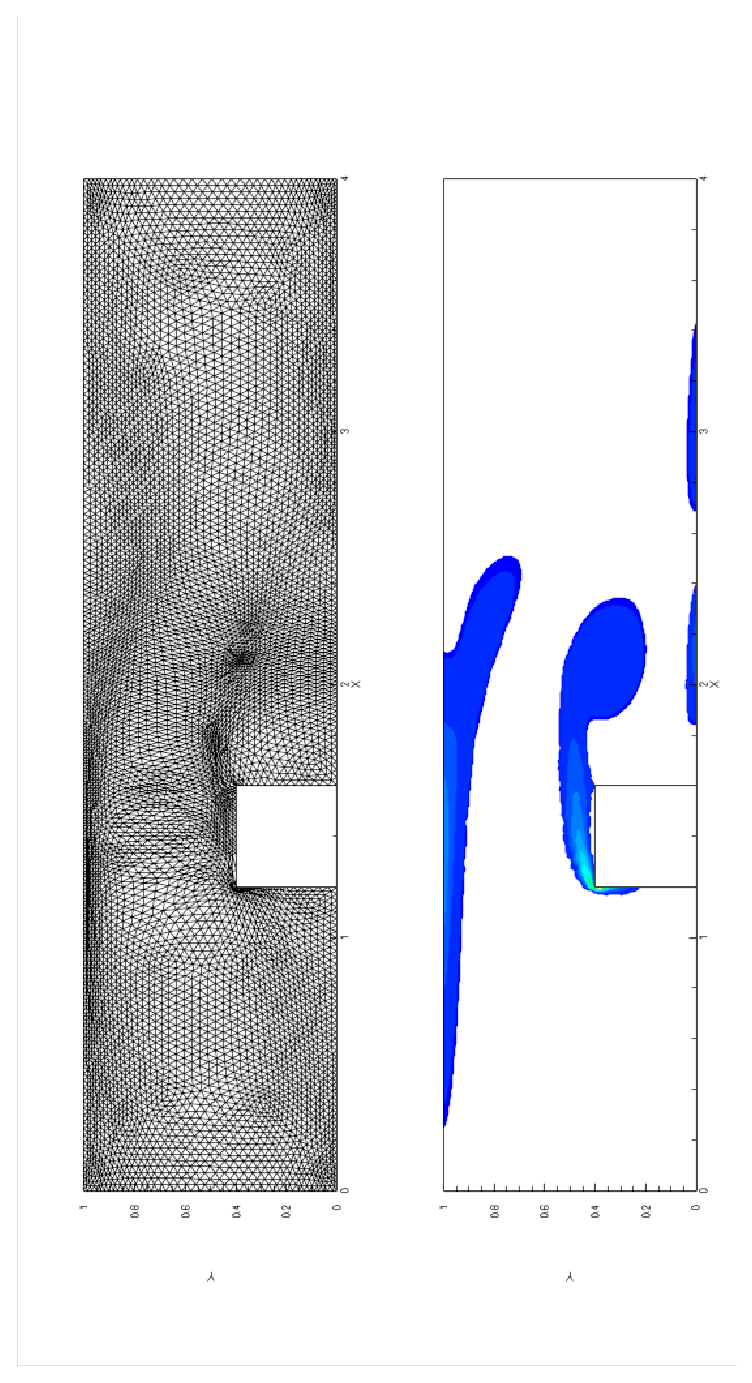
\includegraphics[width = 0.55\textwidth, angle = -90]{picture/step_flow_data/mesh_t_1s.eps}
        \caption{\small Up: moving mesh; bottom: contour of vorticity
          at t = 1s}
        \label{fig::step_flow_1s}
      \end{figure}

      \begin{figure}[!htbp]
        \centering
        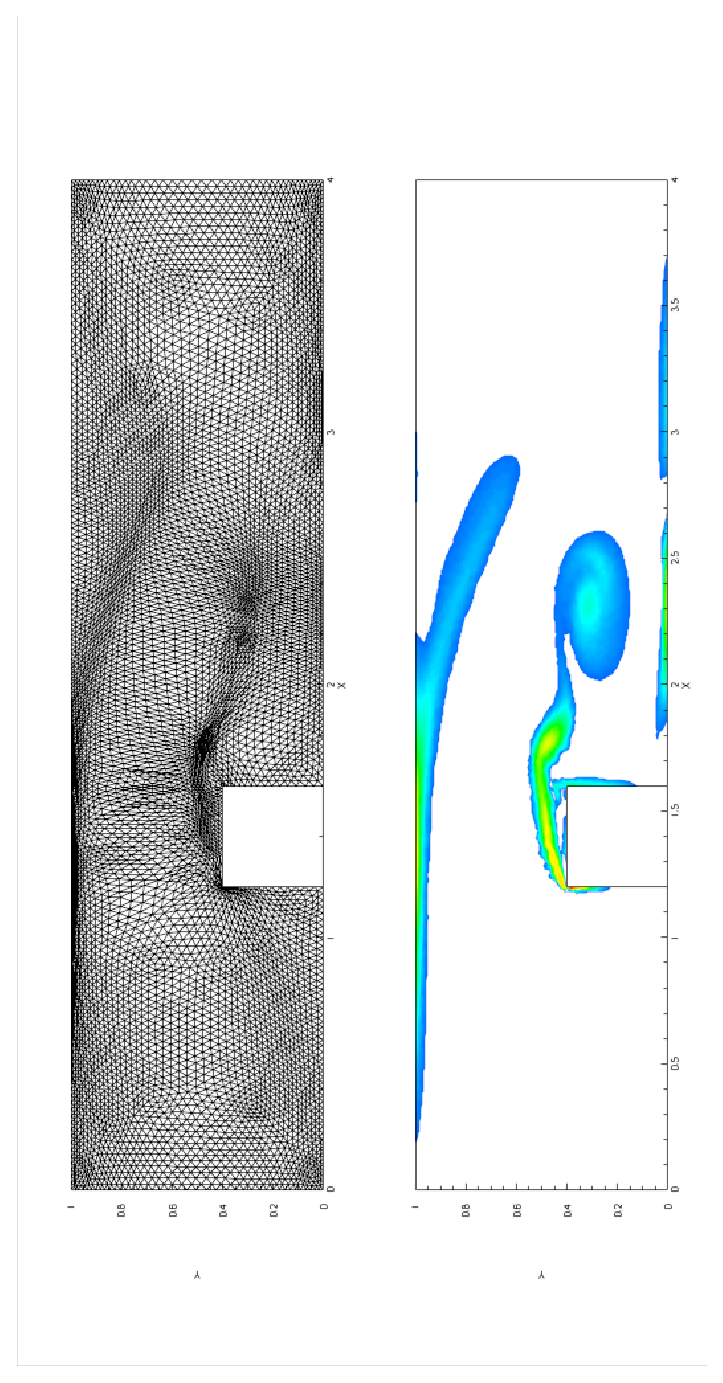
\includegraphics[width = 0.55\textwidth, angle = -90]{picture/step_flow_data/mesh_t_1_5s.eps}
        \caption{\small Up: moving mesh; bottom: contour of vorticity
          at t = 1.5s}
        \label{fig::step_flow_1_5s}
      \end{figure}

      \begin{figure}[!htbp]
        \centering
        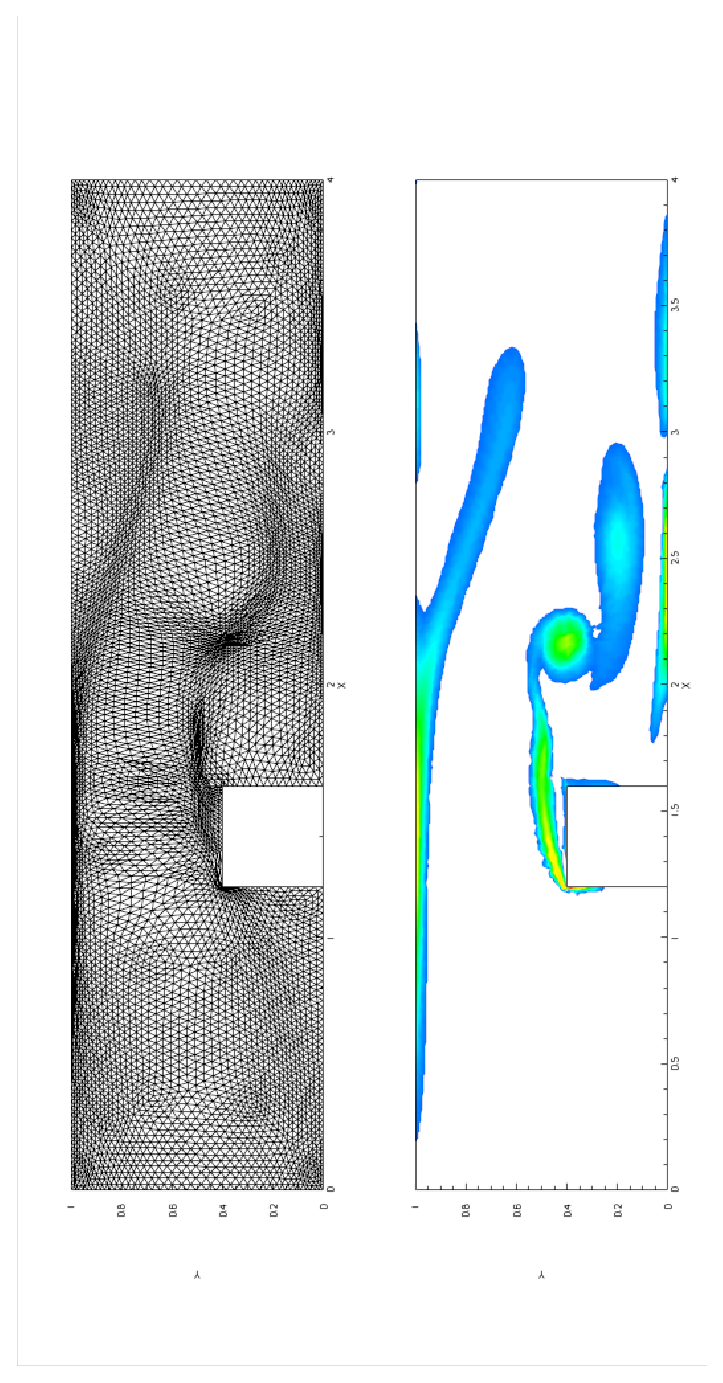
\includegraphics[width = 0.55\textwidth, angle = -90]{picture/step_flow_data/mesh_t_2s.eps}
        \caption{\small Up: moving mesh; bottom: contour of vorticity
          at t = 2s}
        \label{fig::step_flow_2s}
      \end{figure}

      \begin{figure}[!htbp]
        \centering
        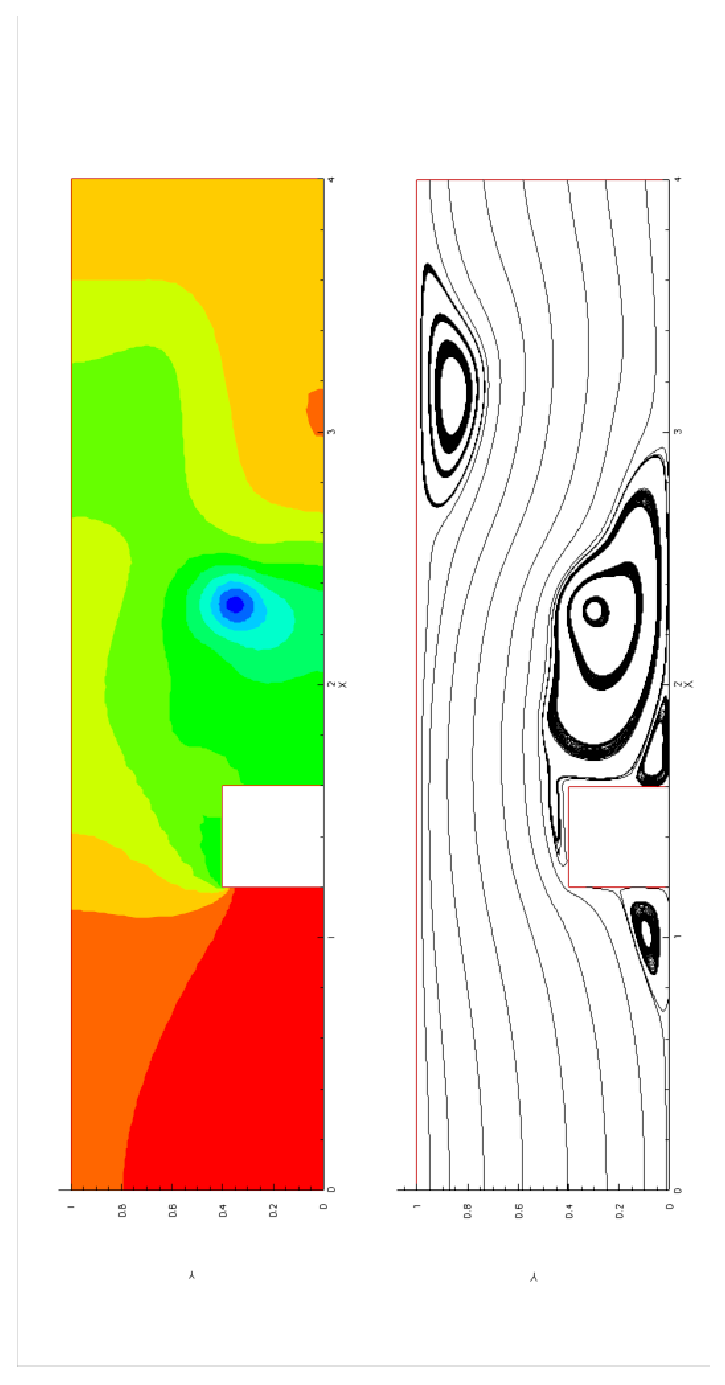
\includegraphics[width = 0.55\textwidth, angle = -90]{picture/step_flow_data/contour_streamline_t_2s.eps}
        \caption{\small Up: Pressure contour; bottom: velocity streamline
          at t = 2s}
        \label{fig::step_flow_contour_streamline_2s}
      \end{figure}

   \subsection{Navier-Stokes flow over cylinder}
   
      This example models the development of flow over an cylinder
      along a retangular channel. In \cite{cao1999anr}, the authors
      apply moving finite element method to this problem. The center
      of cylinder is $(0, 0)$ and radius is $r = 0.3$. Let viscosity
      $nu = 0.003$ and domain $\Omega = [-1, 5] \times [-1, 1]$. 
      Poiseuille flow $u = 1 - y^2, v = 0$ is imposed on inflow
      boundary $x = -1$. $u = v = 0$ is imposed on the top and bottom
      of the channel. Outflow boundary $x = 5$ is natrual
      condition. 

      If we concern the fine flow structure, it is required
      high resolution for small scale structure. For detecting the
      vorticity, (\ref{eq::monitor_vorticity}) is a good choice as the
      monitor in our moving strategy. The parameters $\alpha$ and
      $\beta$ are $1.0$, $2.0$. 

      The evolution of moving mesh and vorticity streamline  
      are illustrated in Figure \ref{fig::cylinder_initial_mesh} and
      Figure \ref{fig::cylinder_mesh_t24_5s}. It
      can be discoverd that our moving mesh can efficiently capture the
      vorticity structure and our mesh quality is better than \cite{cao1999anr}.
      
      When we change the value of viscosity $\nu = 0.001$, the
      structure of moving mesh and vorticity contour are not so
      obvious as viscosity $\nu = 0.003$ as shown in 
      Figure \ref{fig::cylinder_mesh_t23s}. 
      
      \begin{figure}[!htbp]
        \centering
        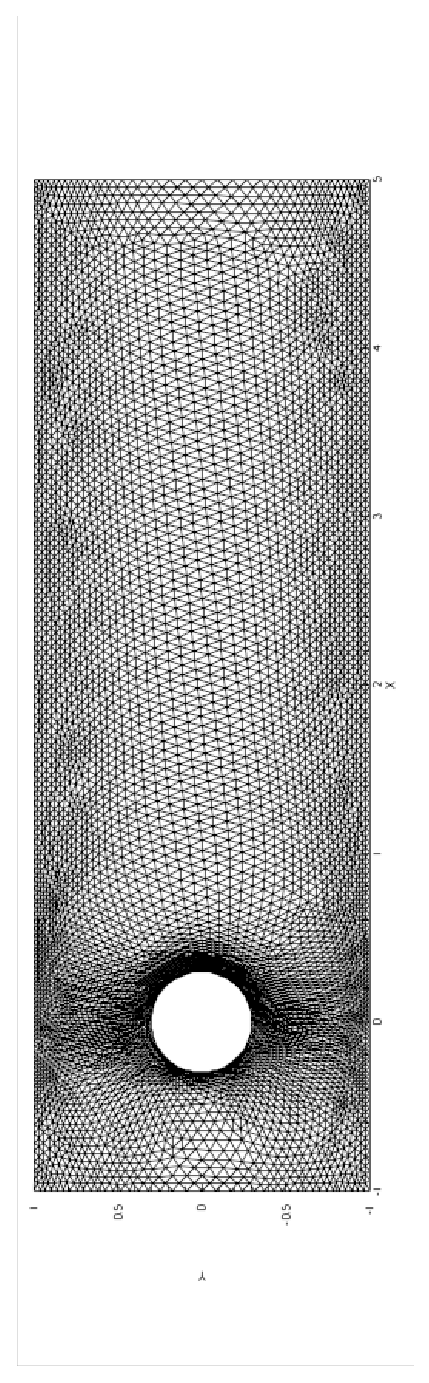
\includegraphics[width = 0.6\textwidth, angle = -90]{picture/obstacle_flow_data/initial_mesh.eps}
        \caption{\small Up: uniform mesh; bottom: initial
          moving mesh, viscosity $\nu = 0.003$.}
        \label{fig::cylinder_initial_mesh}
      \end{figure}

    %   \begin{figure}[!htbp]
    %     \centering
    %     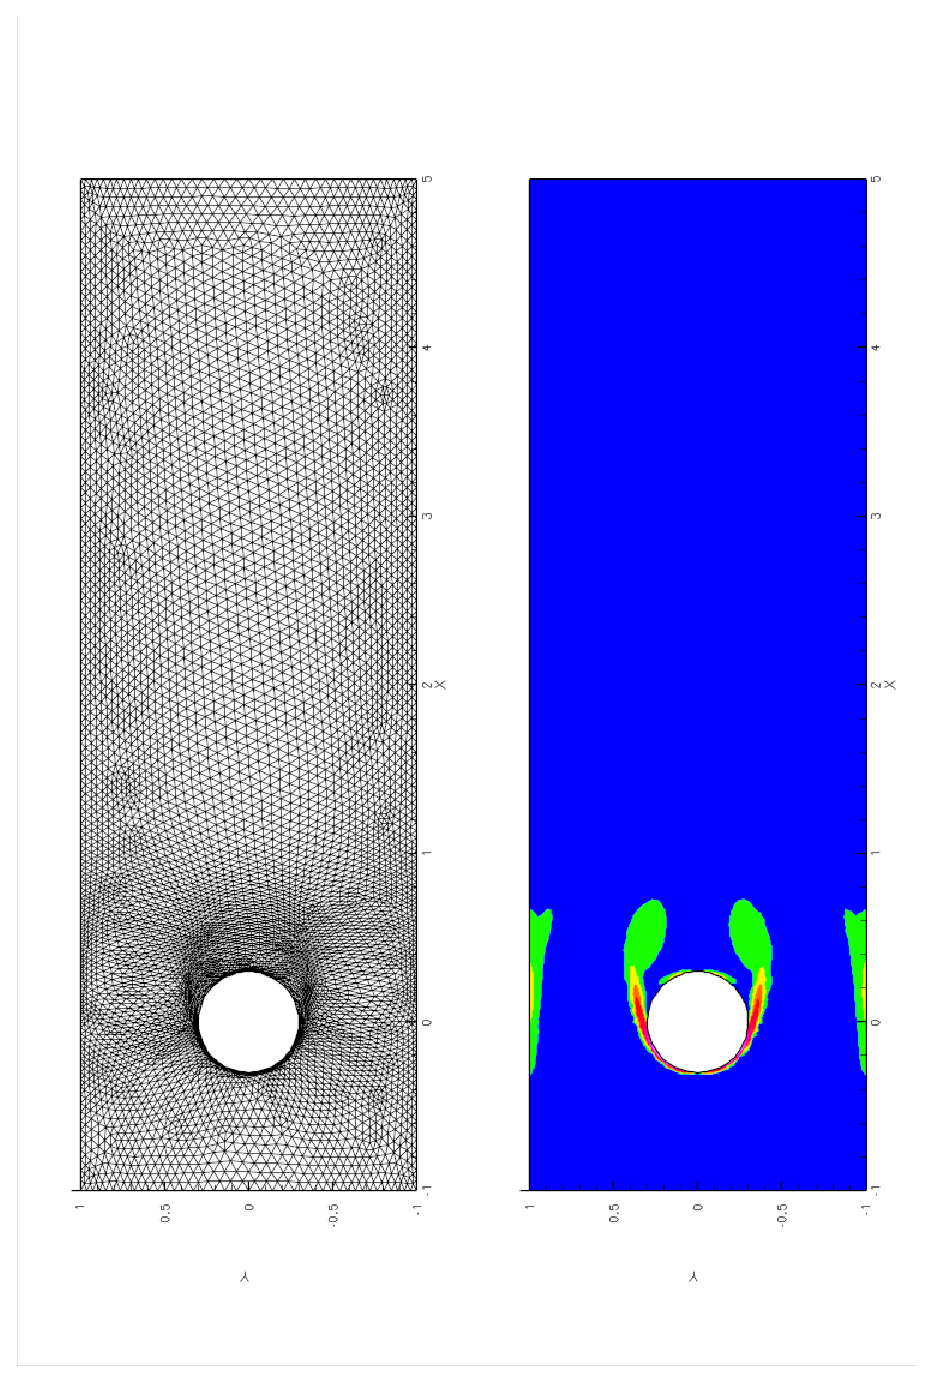
\includegraphics[width = 0.7\textwidth, angle = -90]{picture/obstacle_flow_data/mesh_t_1s.eps}
    %     \caption{\small Up: moving mesh; bottom: vorticity
    %       contour at $t = 1s$.}
    %     \label{fig::cylinder_mesh_t1s}
    %   \end{figure}

    %  \begin{figure}[!htbp]
    %     \centering
    %     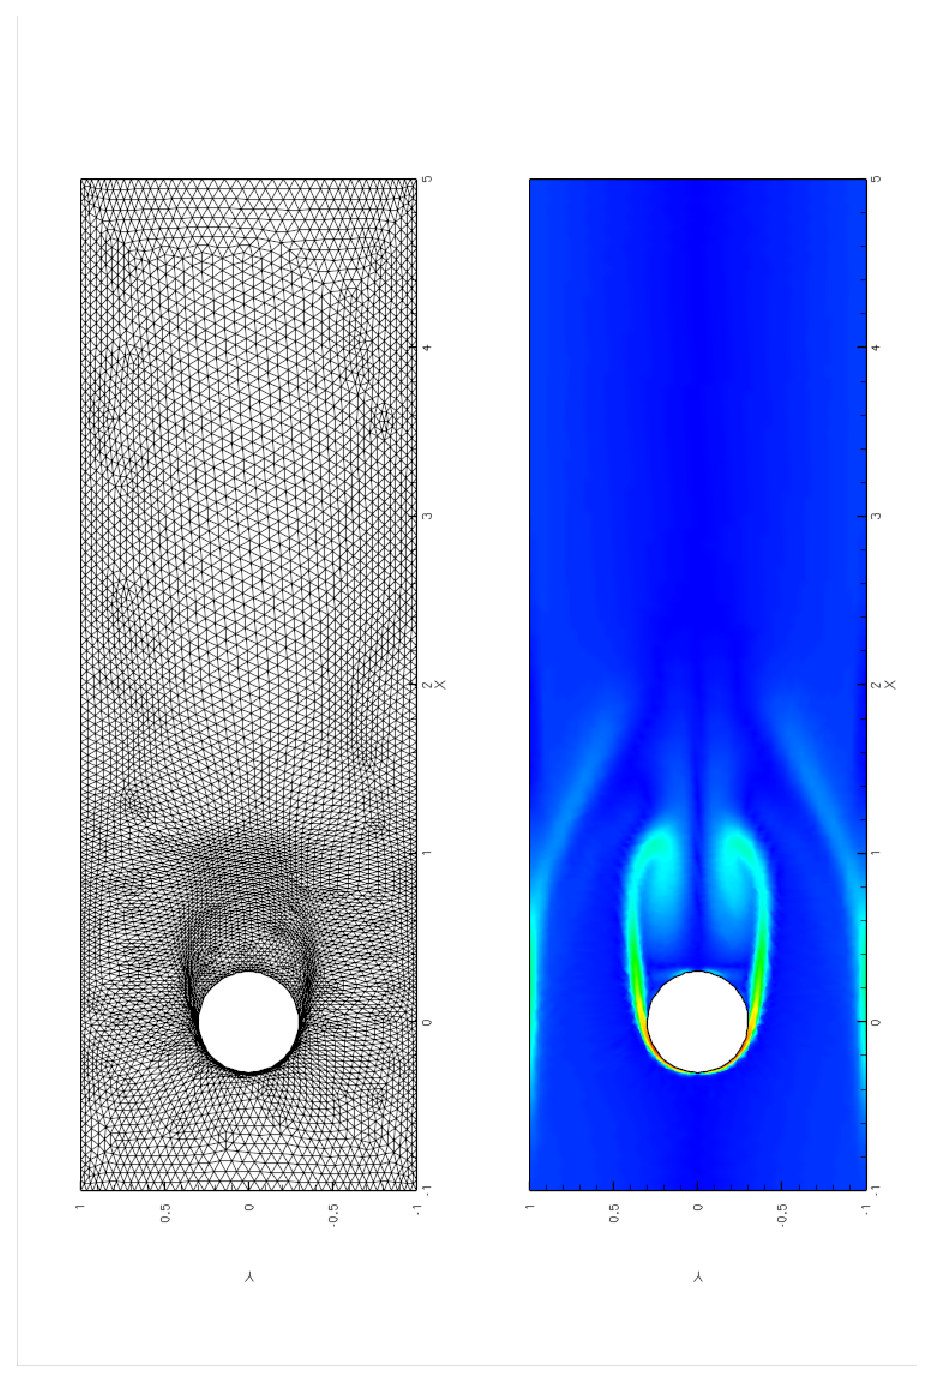
\includegraphics[width = 0.7\textwidth, angle = -90]{picture/obstacle_flow_data/mesh_t_2s.eps}
    %     \caption{\small Up: moving mesh; bottom: vorticity contour at $t
    %       = 2s$.}
    %     \label{fig::cylinder_mesh_t2s}
    %  \end{figure}

    %  \begin{figure}[!htbp]
    %     \centering
    %     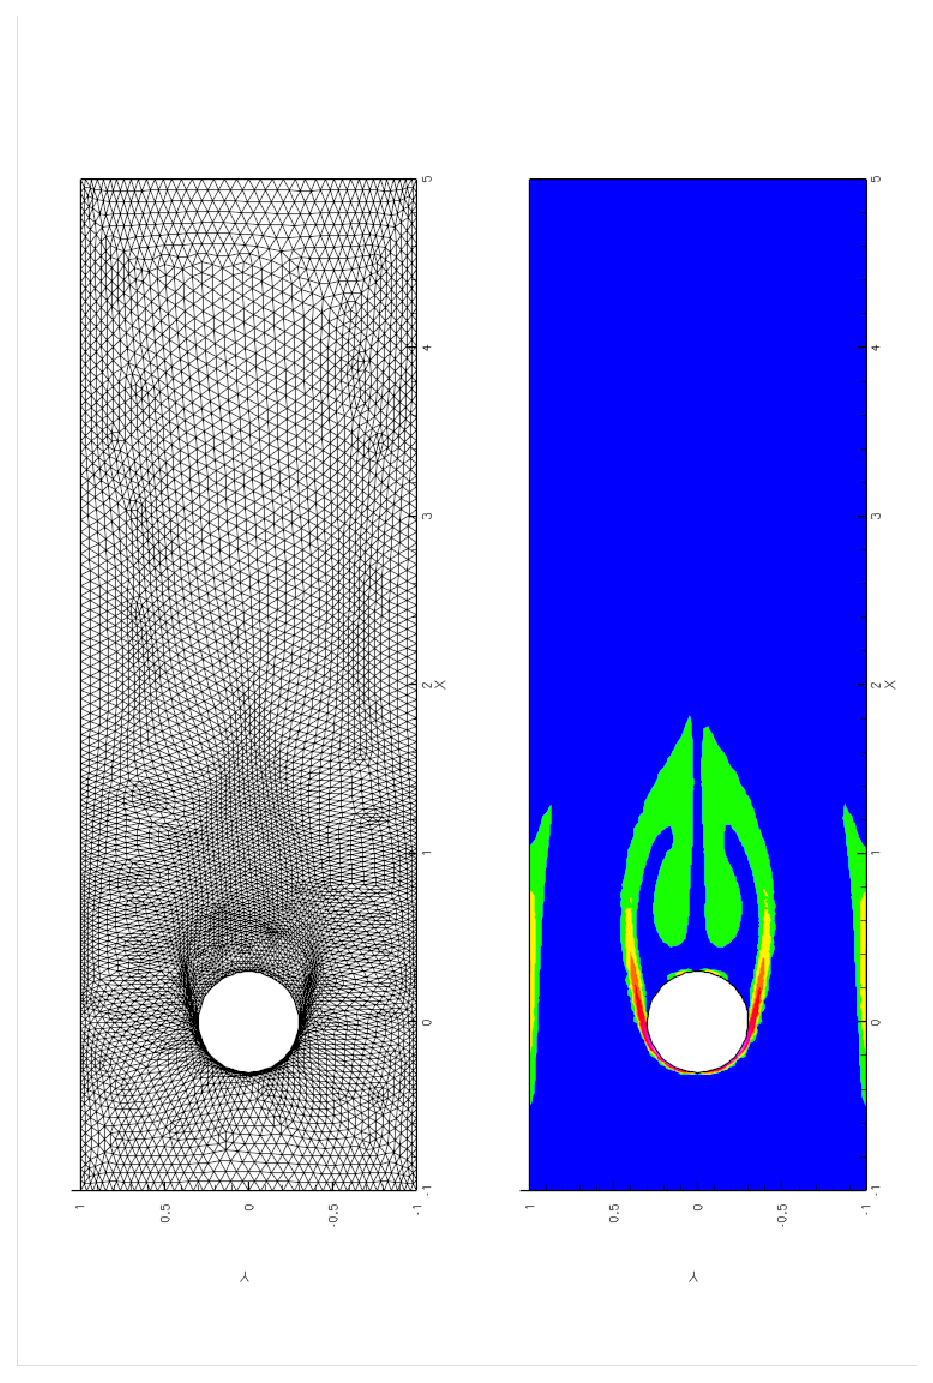
\includegraphics[width = 0.7\textwidth, angle = -90]{picture/obstacle_flow_data/mesh_t_4s.eps}
    %     \caption{\small Up: moving mesh; bottom: vorticity contour at
    %       $t = 4s$.}
    %     \label{fig::cylinder_mesh_t4s}
    % \end{figure}

    \begin{figure}[!htbp]
      \begin{center}
        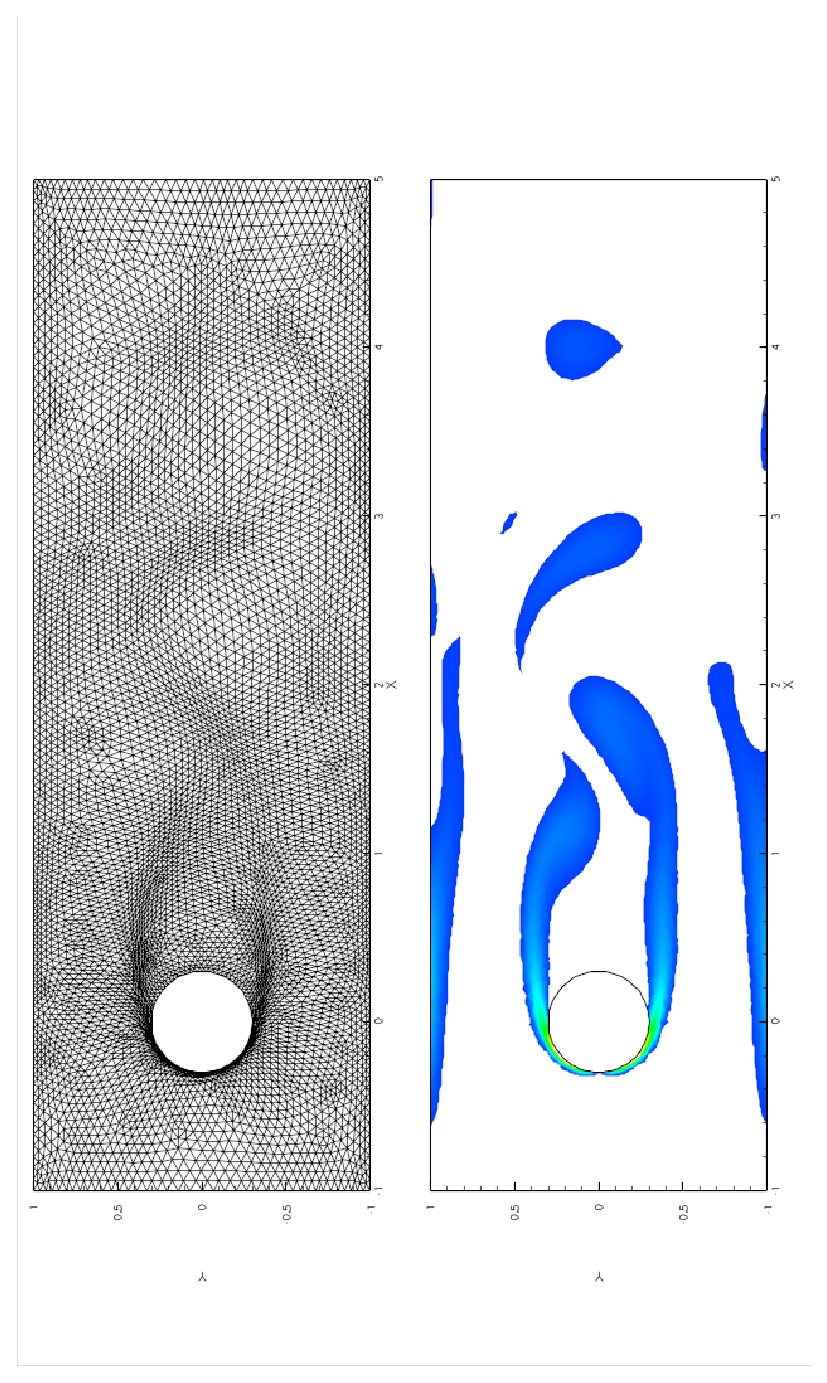
\includegraphics[width = 0.6\textwidth, angle = -90]{picture/obstacle_flow_data/mesh_t_24_5s.eps}
      \end{center}  
      \caption{\small Up: moving mesh; bottom: vorticity contour at
        $t = 24.5s$, viscosity $\nu = 0.003$.}
      \label{fig::cylinder_mesh_t24_5s}
    \end{figure}

    \begin{figure}[!htbp]
        \centering
        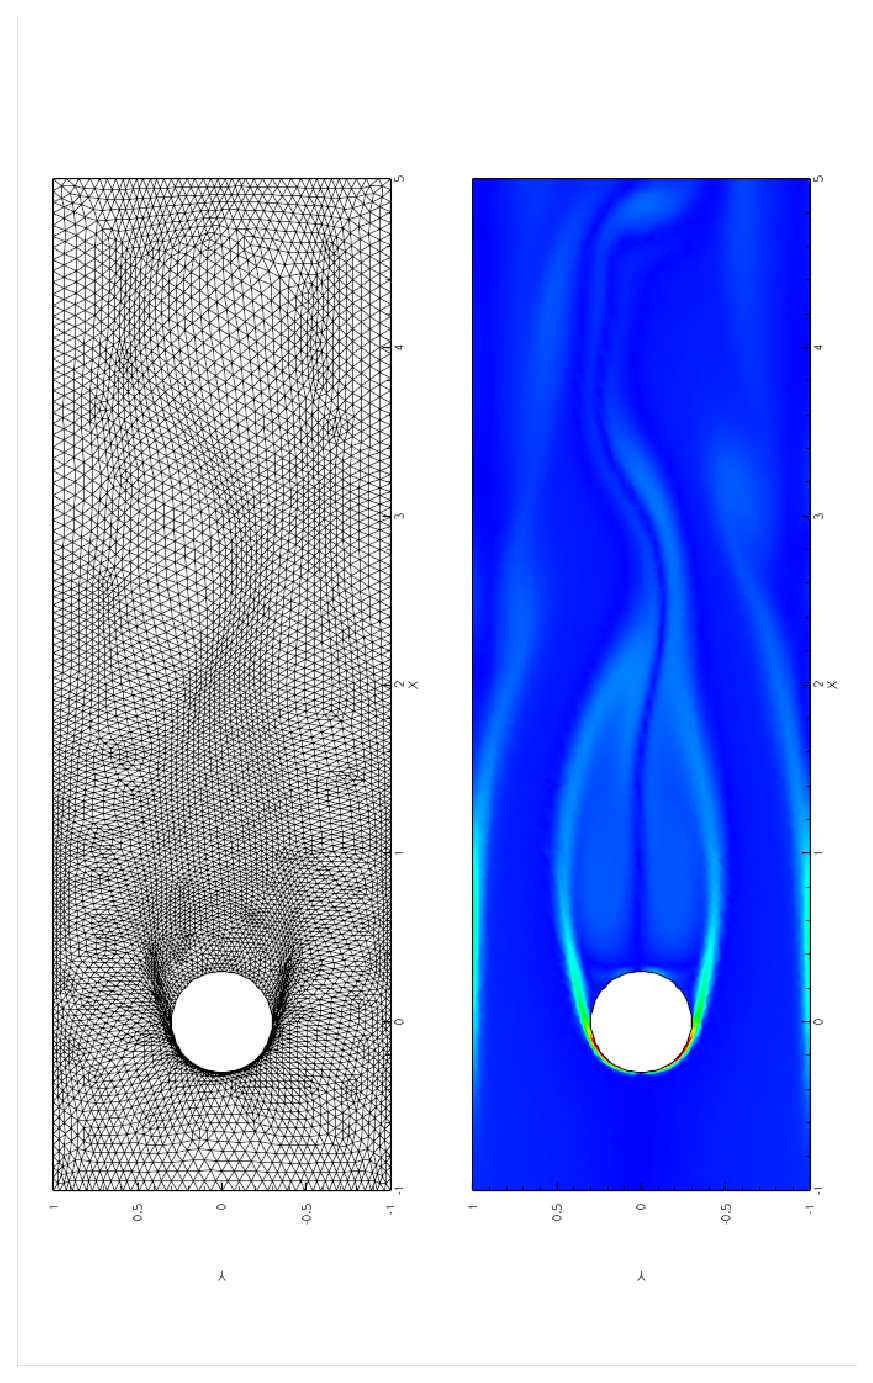
\includegraphics[width = 0.6\textwidth, angle = -90]{picture/obstacle_flow_data/mesh_t_23s.eps}
        \caption{\small Up: moving mesh; bottom: vorticity contour at
          $t = 23s$, viscosity $\nu = 0.001$.}
        \label{fig::cylinder_mesh_t23s}
    \end{figure}

   % ----------------------------------------------------------------------------------------
   %	SECTION 4
   % ----------------------------------------------------------------------------------------

   \section{Remarks}

   In this paper, unsteady Navier-Stokes equations have been numerically 
   solved using moving mesh method on $4P1-P1$ finite element
   pair. The main work is using the hierachy geometry tree structure
   to simply build system matrix by $4P1-P1$ element pair. And we
   apply moving mesh method to this pair. 
    
   $4P1-P1$ element pair natrually satisfies the LBB confiditon and is
   linear-order element. In practical engeneering computation,
   linear-order element is more popular than high order because of its
   simplicity and complexity of problems. For capturing the fine flow
   structure, we apply moving mesh method to this pair using vorticity
   as monitor. The moving mesh is consistent with the structure of
   vorticity. Boundary conditions in our testing problem are all
   non-periodic, so it has more extensive application.
   
   Our mesh structure is based on the hierachy geometry tree
   structure, multi-mesh adaptive method will be applied to $4P1-P1$
   pair. Also moving mesh method for incompressible flow will be
   extended to three-dimention in future work. 
   
   % ----------------------------------------------------------------------------------------
   %	BIBLIOGRAPHY
   % ----------------------------------------------------------------------------------------

   \bibliographystyle{unsrt}

   %% 不知道为何,这里只能用一个bib文件?
   \bibliography{mathpaper} %, mathbook, sample}
   % ----------------------------------------------------------------------------------------


 \end{document}
